%% ****** Start of file apstemplate.tex ****** %
%%
%%
%%   This file is part of the APS files in the REVTeX 4 distribution.
%%   Version 4.1r of REVTeX, August 2010
%%
%%
%%   Copyright (c) 2001, 2009, 2010 The American Physical Society.
%%
%%   See the REVTeX 4 README file for restrictions and more information.
%%
%
% This is a template for producing manuscripts for use with REVTEX 4.0
% Copy this file to another name and then work on that file.
% That way, you always have this original template file to use.
%
% Group addresses by affiliation; use superscriptaddress for long
% author lists, or if there are many overlapping affiliations.
% For Phys. Rev. appearance, change preprint to twocolumn.
% Choose pra, prb, prc, prd, pre, prl, prstab, prstper, or rmp for journal
%  Add 'draft' option to mark overfull boxes with black boxes
%  Add 'showpacs' option to make PACS codes appear
%  Add 'showkeys' option to make keywords appear
\documentclass[aps,pra,notitlepage,groupedaddress]{revtex4-1}
%\documentclass[aps,prl,preprint,superscriptaddress]{revtex4-1}
%\documentclass[aps,prl,reprint,groupedaddress]{revtex4-1}

% You should use BibTeX and apsrev.bst for references
% Choosing a journal automatically selects the correct APS
% BibTeX style file (bst file), so only uncomment the line
% below if necessary.
%\bibliographystyle{apsrev4-1}

\usepackage[margin=1.5in]{geometry}

\usepackage{graphicx}
\usepackage{amsmath}
\usepackage{subcaption}
\usepackage{hyperref}
\usepackage{color}

\captionsetup[figure]{justification=raggedright,singlelinecheck=false}
\captionsetup[subfigure]{justification=centering,singlelinecheck=false}
\captionsetup[table]{justification=raggedright,singlelinecheck=false}

\begin{document}
%\linenumbers
% Use the \preprint command to place your local institutional report
% number in the upper righthand corner of the title page in preprint mode.
% Multiple \preprint commands are allowed.
% Use the 'preprintnumbers' class option to override journal defaults
% to display numbers if necessary
%\preprint{}

%Title of paper
\title{Global Quantum Efficiency Simulation with RAT}

% repeat the \author .. \affiliation  etc. as needed
% \email, \thanks, \homepage, \altaffiliation all apply to the current
% author. Explanatory text should go in the []'s, actual e-mail
% address or url should go in the {}'s for \email and \homepage.
% Please use the appropriate macro foreach each type of information

% \affiliation command applies to all authors since the last
% \affiliation command. The \affiliation command should follow the
% other information
% \affiliation can be followed by \email, \homepage, \thanks as well.
\author{Thomas Wester \\ \small{\href{https://github.com/tbwester/ratpac-nudot/}{https://github.com/tbwester/ratpac-nudot/}}}

%\email[]{Your e-mail address}
%\homepage[]{}
%\thanks{}
%\altaffiliation{}
\affiliation{}

%Collaboration name if desired (requires use of superscriptaddress
%option in \documentclass). \noaffiliation is required (may also be
%used with the \author command).
%\collaboration can be followed by \email, \homepage, \thanks as well.
%\collaboration{}
%\noaffiliation

\date{\today}

\maketitle

\tableofcontents

\section{Introduction}

This note describes the optical photon simulation created to accompany measurements made with MicroBooNE PMTs in the Bo cryostat. The purpose of the measurements is to determine the global quantum efficiency (GQE) of the MicroBooNE optical units, which consist of a wavelength-shifting plate and a photomultiplier tube (PMT). A measurement for the GQE was determined by measuring an observed quantity of photoelectrons (PEs) from the PMT, combined with an estimate of the number of photons which hit the plate, corresponding to that particular PE number. The GQE, then, is:

\begin{equation}\label{eq:gqe}
\text{GQE} \equiv \langle Q \rangle = \frac{\text{\# PE}}{\text{\# Photons Hits on the Plate}}
\end{equation}

Data was taken using a Polonium alpha source which is estimated to produce $134000 \pm 6000$ photons per decay in liquid argon. This source holder was placed at two distances away from the plate, $d=20.3$cm and $d=36.8$cm.

This simulation uses RAT, a software package based around GEANT4, to handle the ray tracing and the interactions of photons with the various materials in the cryostat. The objective of the simulation is to confirm the PE measurement made previously, and determine a value for the corresponding number of photons which hit the TPB plate at both $d$ positions of the source.

%The simulation is divided into two steps: First, 128nm light is simulated as originating from scintillation in liquid argon induced by an alpha source. This light is propagated to an acrylic plate with a wavelength-shifting TPB coating. The position of the hits on this plate are saved. Second, 420nm light (representing wavelength-shifted photons) is created within the TPB plate and tracked through a glass volume representing the window of a MicroBooNE PMT. Photons which make it through this glass volume are recorded as successful hits.

\section{Geometry}

The Bo optical photon simulation uses the following convention: the positive $z$-direction points from the top of the cryostat towards the bottom, where the TPB plate and PMT are located. The $x$-$y$ plane is perpendicular and azimuthal symmetry is assumed (although the simulation is fully 3-D) for some analyses. The origin is placed at the center (depth-wise and width-wise) of the cryostat volume. Every quantity listed in inches is converted to centimeters with the factor $2.54$. An overview of the geometry is shown in Figure \ref{fig:geo}.

\begin{figure}
	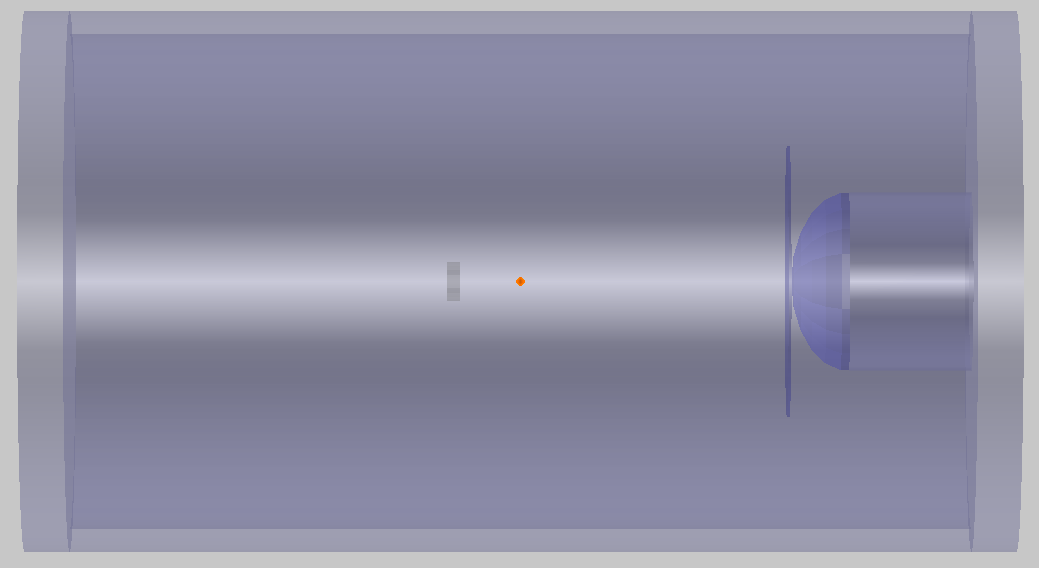
\includegraphics[width=1.0\textwidth]{figures/geo_overview}
	\caption{A view of the simulated Bo cryostat geometry showing (from left to right) the source holder, TPB plate, PMT glass and PMT metal shield. The origin in the simulation coordinate system is the orange point. \label{fig:geo}}
\end{figure}

\subsection{The Bo Cryostat}

The Bo cryostat is a cylindrical volume 40 inches in depth and 11 inches in inner-radius. Two end caps are placed with inner faces at $z=\pm 20$ inches to enclose the volume. 

\subsection{Source Holder}

The source holder is centered in the $x$-$y$ plane and is varied in position along the $z$-axis. The holder is modeled using two stacked ring volumes and an additional solid cylinder. A cross section is shown in Figure \ref{fig:holder}. The top two rings total in height to form the source collimator. The source itself is placed 0.01mm above the back of the collimator to simulate (i) the thickness of the aluminum foil on which the polonium is deposited and (ii) the potential for backscatters of photons reflecting on the aluminum.

There are two sets of measurements for the source holder. The first set, henceforth the ``primary'' set, as reported by Ben Jones, has the height of the inner chamber at 0.09375 inches. The second configuration, measured by Fermilab radiation staff, has this same height at 0.1 inches. In either case, the total depth of the collimator (0.15625") is the same. Additionally, the second set has slightly wider collimator radii, at $2.58$ mm and $3.18$ mm respectively. The effect of switching the geometry configuration is discussed in Section \ref{ssec:system}.

\begin{figure}
	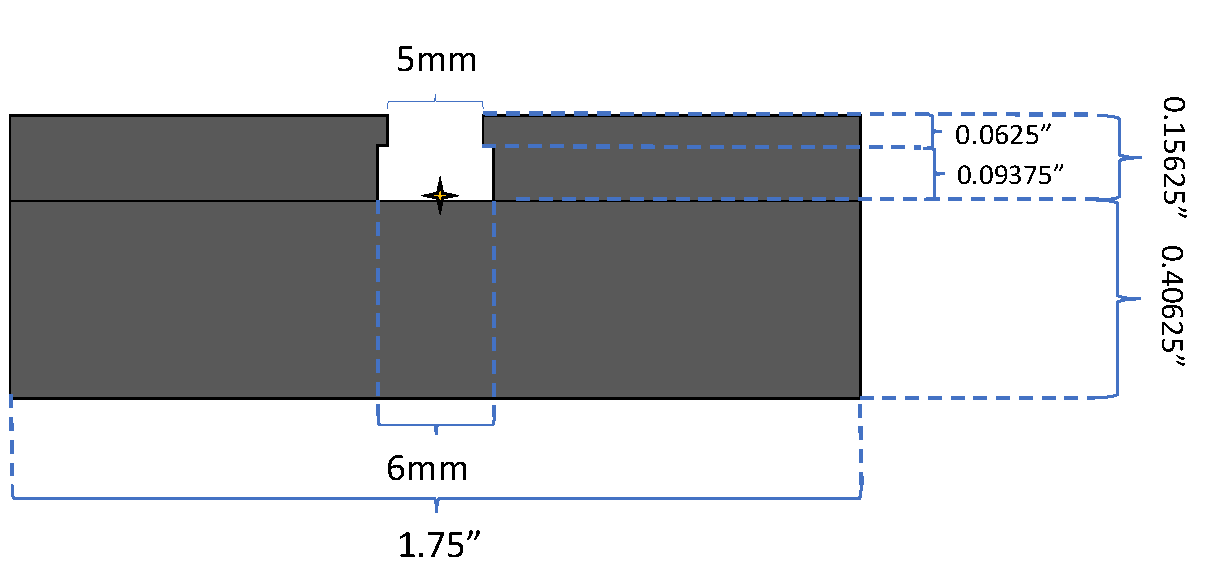
\includegraphics[width=1.0\textwidth]{figures/holder}
	\caption{To-scale cross-section of the source holder, with relevant dimensions labeled, using the primary source holder configuration. The source, a point indicated with a star, is placed just above the back of the collimator. \label{fig:holder}}
\end{figure}

\subsection{TPB Plate \& PMT}

The TPB plate is an acrylic disk 15.24 cm. The plate is placed with its center at the origin in the $x$-$y$ plane and at a fixed position of $z=30$cm (front face). The PMT is modeled as a hollow ellipsoid with minor axis pointing along the $z$-direction at $65$mm in length. The major axes in the $x$ and $y$-directions are identical with length at $101$mm. The thickness of the ellipsoid is 0.5mm throughout. The PMT position is set according to the back face of the TPB plate, such that the closest point of the ellipsoid is 1/8 inch away from the back face of the TPB plate.

The geometry parameters for each detector component are summarized in Table \ref{tab:geo}.

\begin{table}
	\begin{center}
		\begin{tabular}{| c | c | c |}
			\hline
			Quantity	&	Value	&	-	\\
			\hline
			Cryostat Inner Radius	&	11"	&	-	\\
			Cryostat Depth & 40" & - \\
			Collimator Depth 1	&	0.0625"	&	-	\\
			Collimator Depth 2	&	0.09375"	&	-	\\
			Collimator Radius 1 & 2.5 mm & - \\
			Collimator Radius 2 & 3mm & - \\
			TPB Plate Radius & 12" & - \\
			TPB Plate Depth & 0.125" & - \\
			PMT Glass Thickness & 0.5mm & - \\
			PMT Glass Major Axis & 101mm & - \\
			PMT Glass Minor Axis & 65mm & - \\
			\hline
		\end{tabular}
		\caption{Summary of relevant geometry parameters and associated uncertainties (where applicable). Note that the collimator has two associated radii and depths, see Figure \ref{fig:holder}. \label{tab:geo}}
	\end{center}
\end{table}

\subsection{Material Parameters}

Table \ref{tab:mats} lists each simulation feature, its material, and the associated index of refraction, $N$, and reflectivity, $R$. Note that $N$ and $R$ have different values depending on the wavelength of the incident photon.

\begin{table}
	\begin{center}
		\begin{tabular}{| c | c | c | c |}
			\hline
			Feature & Material & $N$ (128/420nm) & $R$ (128/420nm) \\
			\hline
			Source Holder & Aluminum & - & $0.2 \pm 0.1$ \cite{johnson_1968} / - \\
			Cryostat Walls & Stainless Steel & - & 0.35 / $0.540 \pm 0.005$ \cite{nasa} \\
			Cryostat Interior & LAr & $1.45 \pm 0.07$ \cite{grace_butcher_monroe_nikkel_2017} / $1.23 \pm 0.002$ \cite{sinnock_smith_1969} & -\\
			TPB Plate & Acrylic & - / $1.49 \pm 0.2$ \cite{sinnock_smith_1969} & - \\
			PMT Window & Glass & - / $1.46 \pm 0.04$ \cite{malitson_1965}& - \\
			\hline
		\end{tabular}
		\caption{Summary of material properties relevant to the optical simulation. Note that some values are omitted if they are negligible: light produced in the TPB plate is unlikely to reflect on the aluminum source holder. The PMT is not sensitive to 128 nm light, so $N_{\text{Glass}}$ is not used in this simulation for that wavelength. \label{tab:mats}}
	\end{center}
\end{table}

Additionally, we assign the Rayleigh scattering length parameter in LAr as $\lambda=60 \pm 6$ cm \cite{grace_butcher_monroe_nikkel_2017}. The absorption length for pure liquid argon is greater than 1 km \cite{jones_chiu_conrad_ignarra_katori_toups_2013}, and therefore is not relevant to this test.

\section{Analysis \& Results}

The simulation consists of two steps to imitate the wavelength-shifting effect of the TPB plate. The first step propagates 128nm photons from the source holder to the plate, while the second step propagates 420nm photons from the plate to the PMT. The analysis consists of general physics checks, and the creation of a simulated PE spectrum by combining the two simulation steps.

\subsection{Rayleigh Scattering}

Rayleigh scattering has two properties relevant to the optical simulation. First, the probability of scattering is exponential with parameter $\lambda$. Second, the distribution of scattering angles, $\theta_s$, is proportional to $1+\cos^2 \theta_s$.

Both of these properties are implemented within RAT. To test them, we save the initial position and direction of each photon as well as the position and and direction at the instance of first scattering. We can then examine the distributions of the scattering lengths and scattering angle dot product, and fit these distributions to the expected functional form. This is shown in Figure \ref{fig:rayleigh}.

\begin{figure}
	\begin{minipage}{0.49\textwidth}
		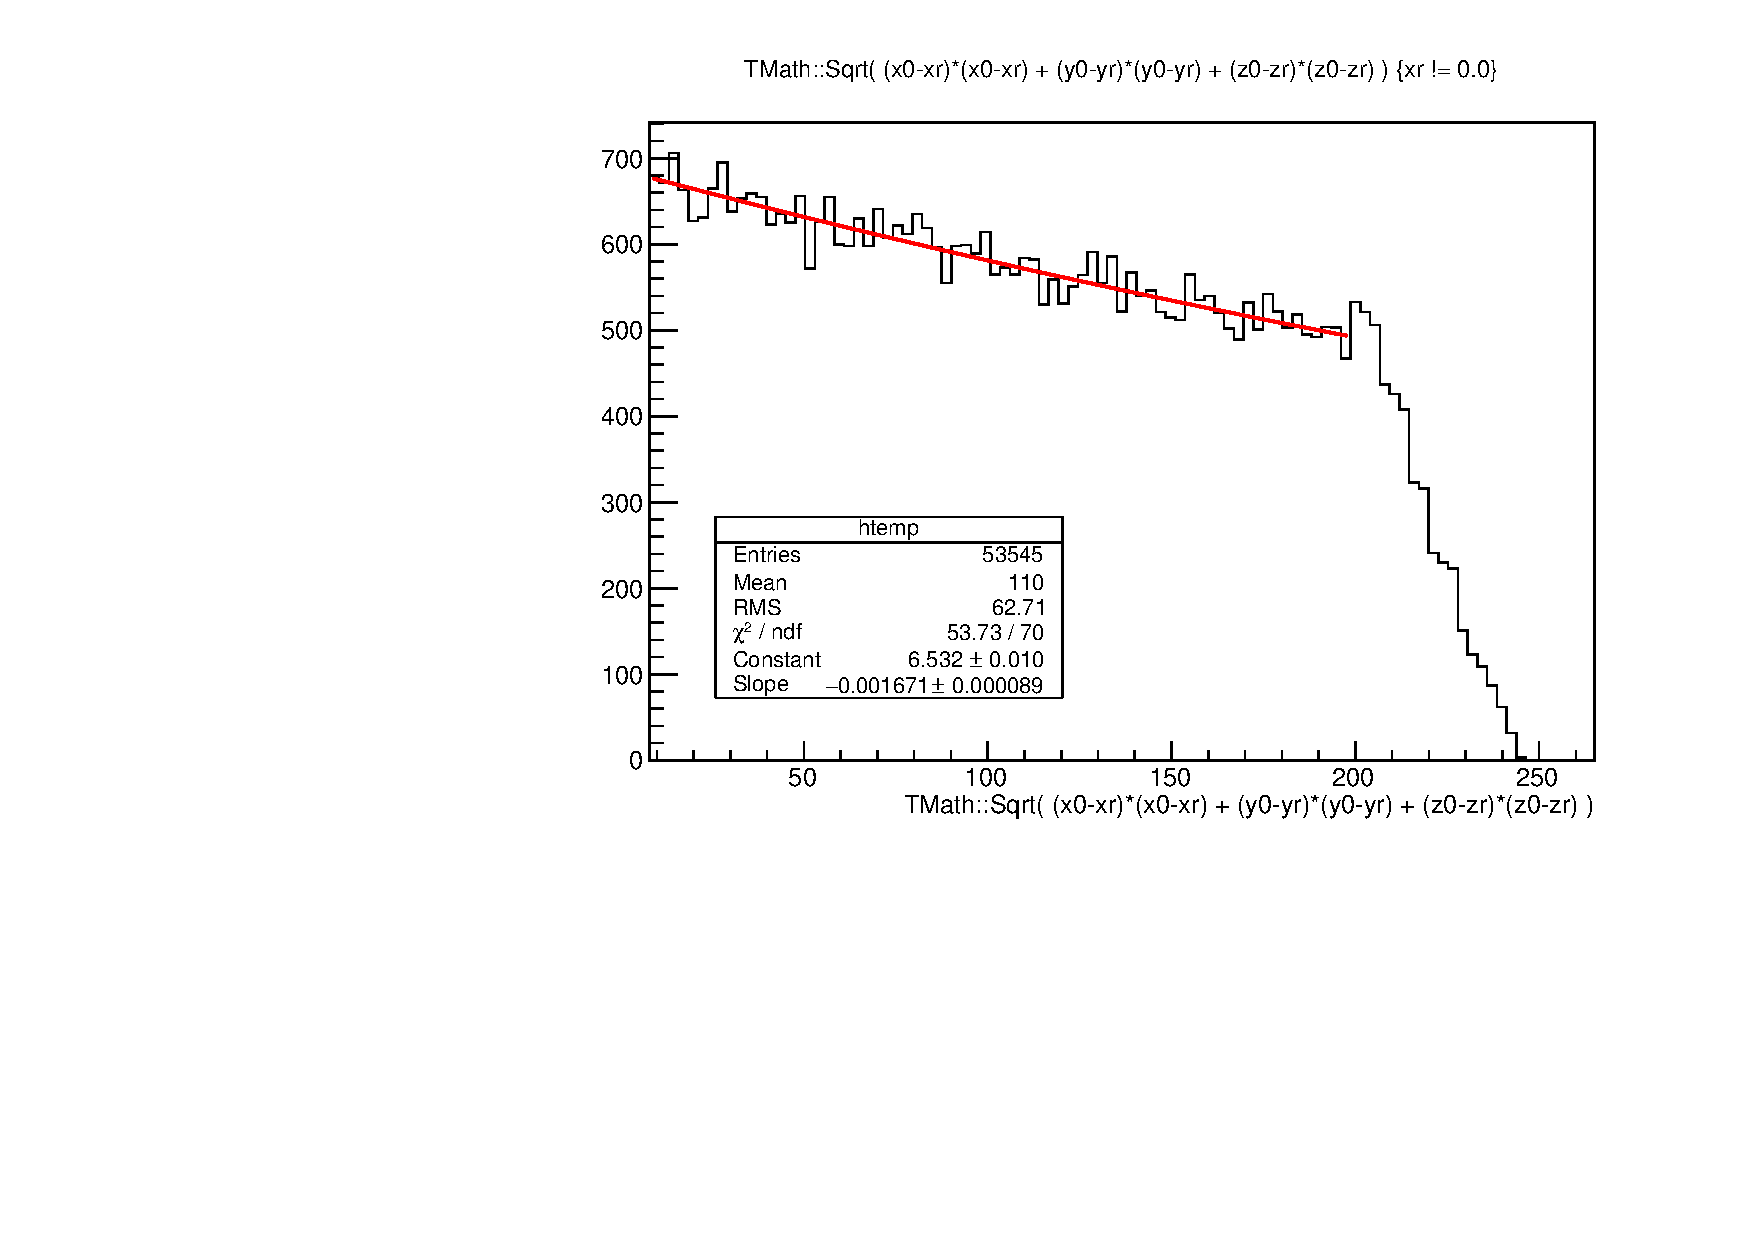
\includegraphics[width=1.0\textwidth]{figures/rlen}
	\end{minipage}
	\begin{minipage}{0.49\textwidth}
		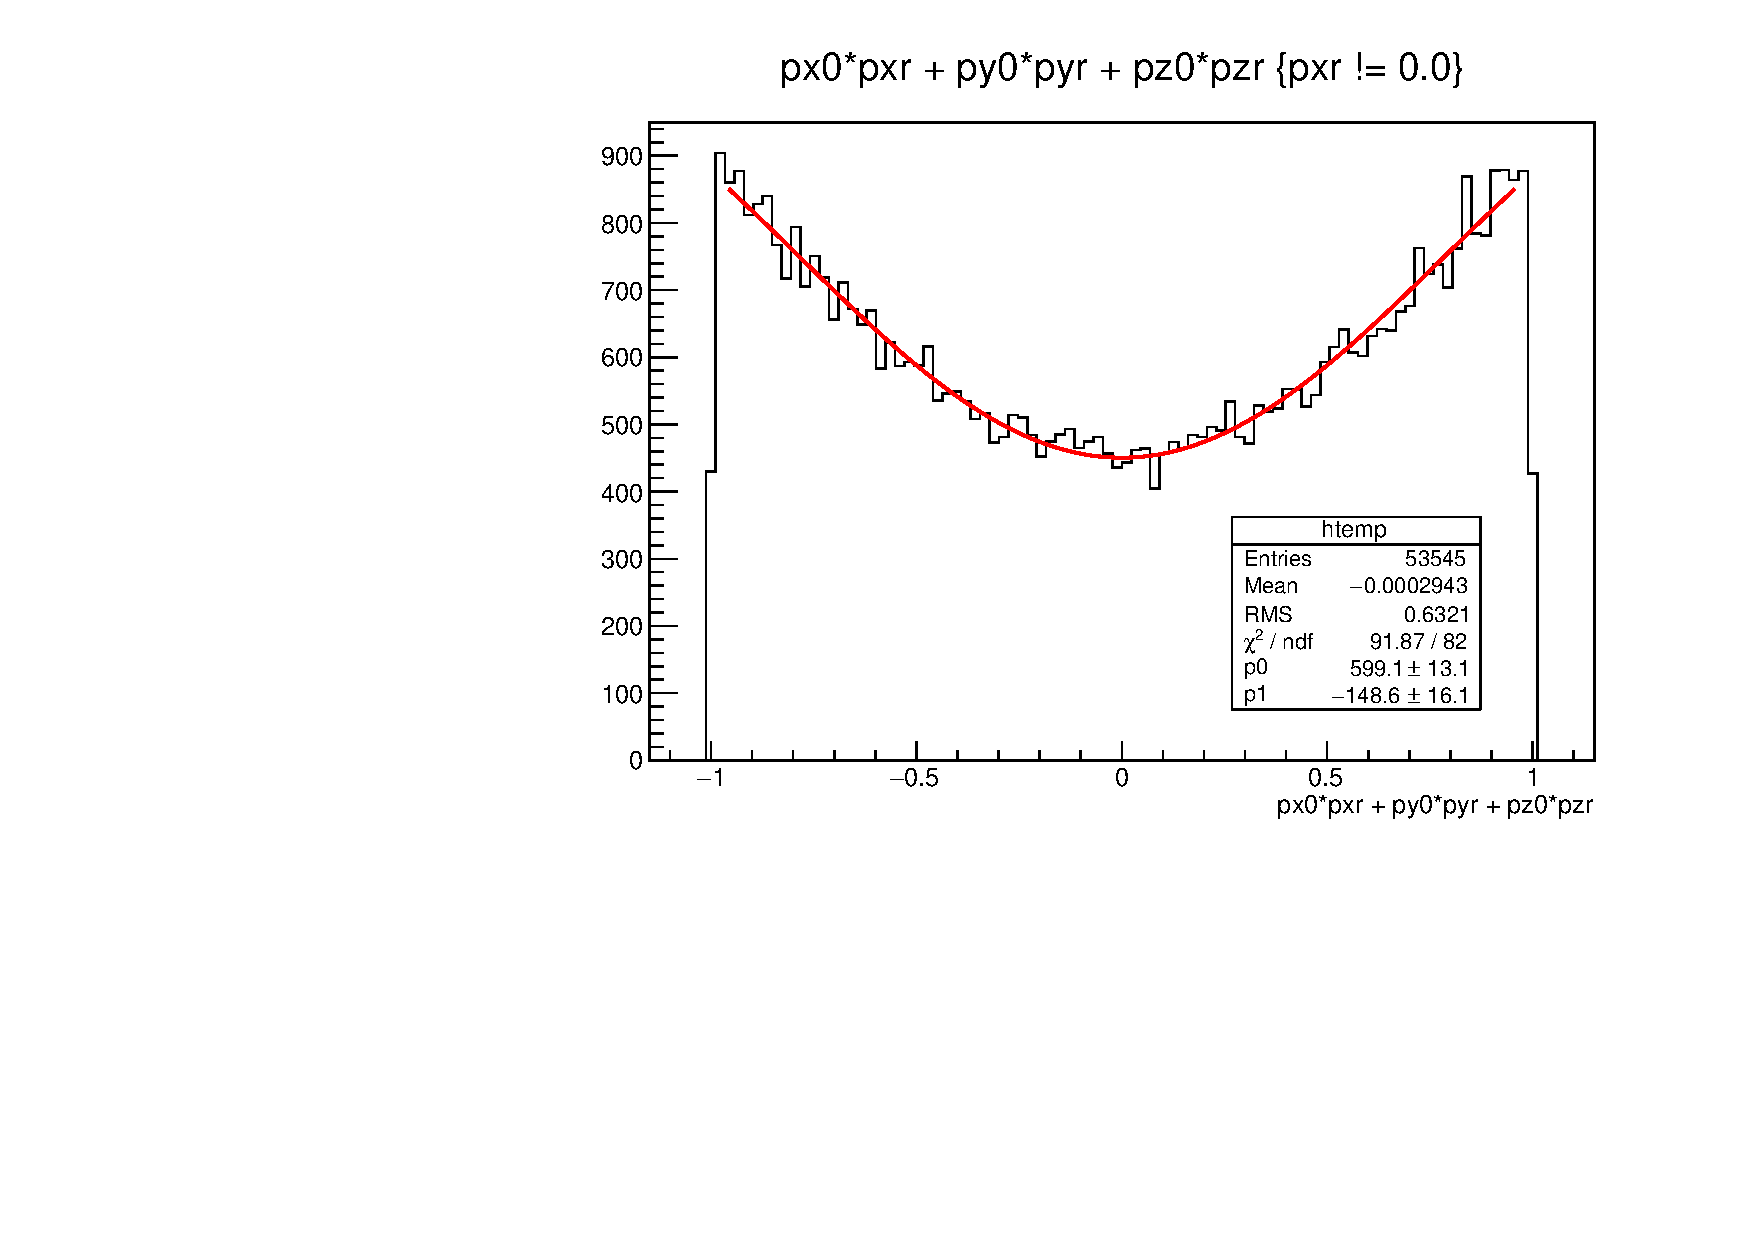
\includegraphics[width=1.0\textwidth]{figures/rthetadist}
	\end{minipage}
	\caption{Left: Exponential function fitted to the distance between photon starting points and corresponding locations of Rayleigh scattering, showing good agreement with the parameter $\lambda = 60$ cm (Note: the fit parameters are in units of mm, and ROOT is fitting the form $\exp[1/\lambda]$. The drop in events at high distances is due to photons hitting the detector walls, etc.). Right: Dot product of initial photon direction with direction after Rayleigh scattering, fitted with a $1+\cos^2\theta$ distribution, also showing good agreement. \label{fig:rayleigh}}
\end{figure}

\subsection{Reflectivity}

We assign a nominal value of 0.10 for the reflectivity of aluminum \cite{johnson_1968}. We can check the initial direction of photons to see the effect of this parameter on the observed number of TPB plate hits. In Figure \ref{fig:reflect}, we show the number of hits as a function of the cosine of the starting angle, $\cos \theta_0$, i.e. the direction the photon is pointing along the $z$-axis. The photon source was placed centered on the $x$-$y$ axis for this test. A cut selecting only those events with negative $\cos \theta_0$, and that did not undergo scattering, gives 12000 events, out of the total 123000 events. This is consistent with the set reflectivity value, noting the asymmetry of the collimator chamber (see Figure \ref{fig:holder}).

\begin{figure}
	\begin{center}
		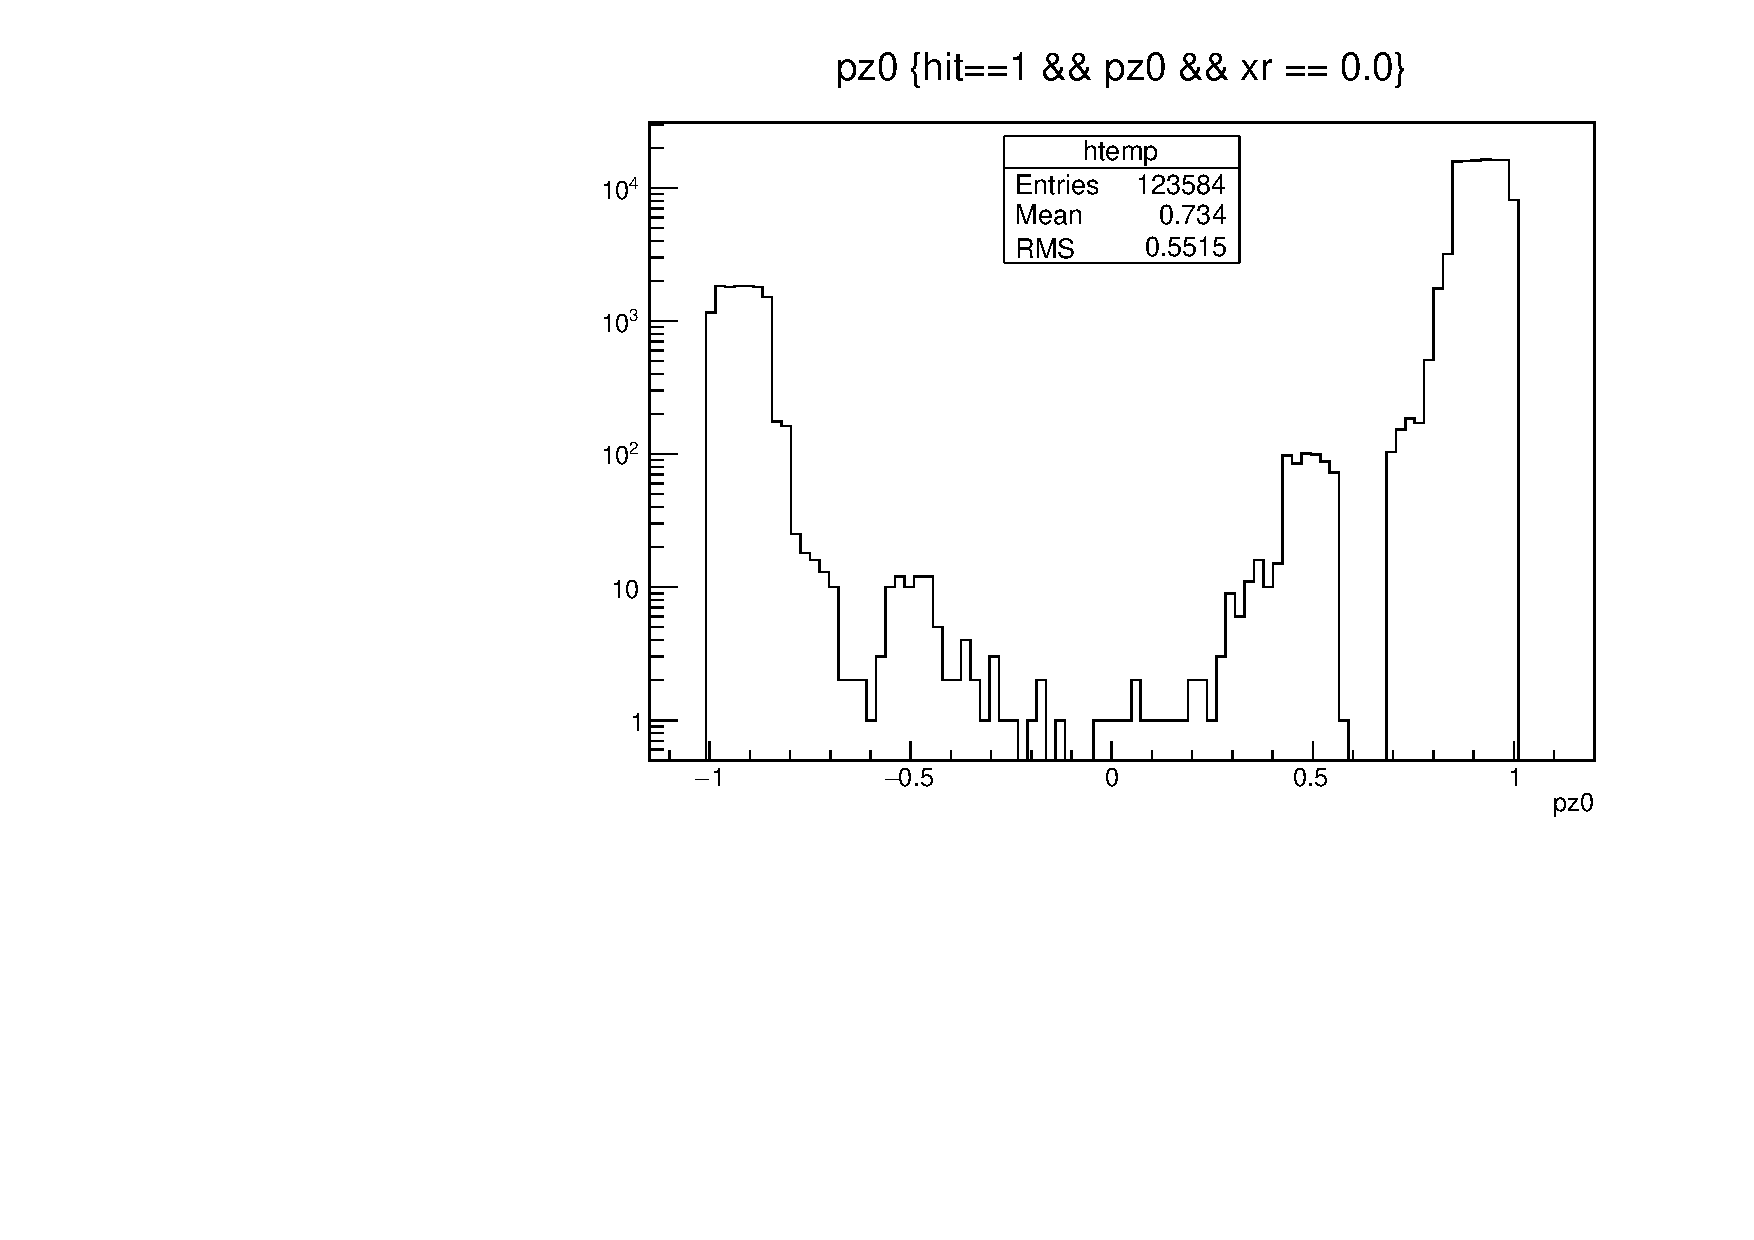
\includegraphics[width=0.7\textwidth]{figures/reflect}
	\end{center}
	\caption{Log-scale plot showing the angular distribution of photons from the source holder which hit the TPB plate.\label{fig:reflect}}
\end{figure}

\subsection{Source to PMT Simulation}

\begin{figure}
	\begin{center}
	\begin{subfigure}{0.32\textwidth}
		\begin{minipage}{1.0\textwidth}
			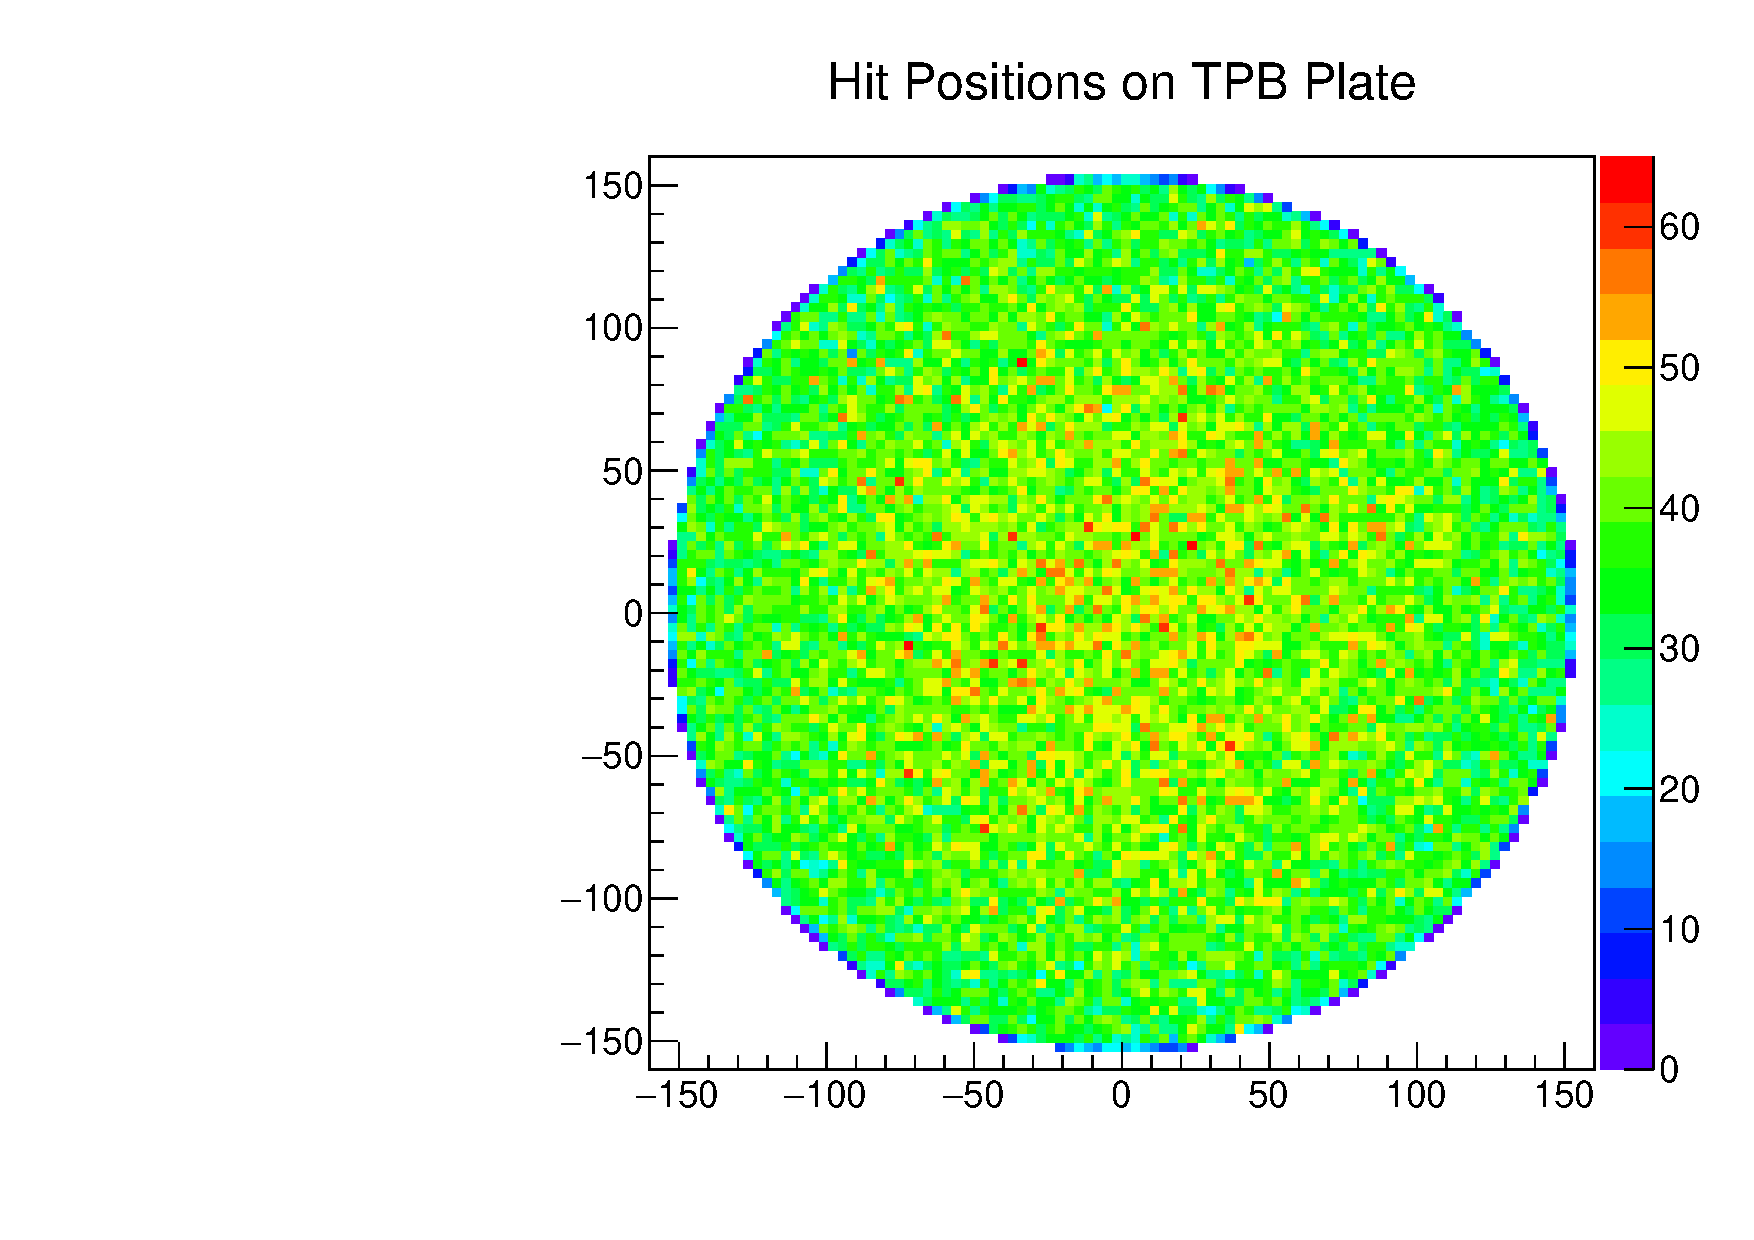
\includegraphics[width=1.0\textwidth]{figures/hit_0.pdf}
			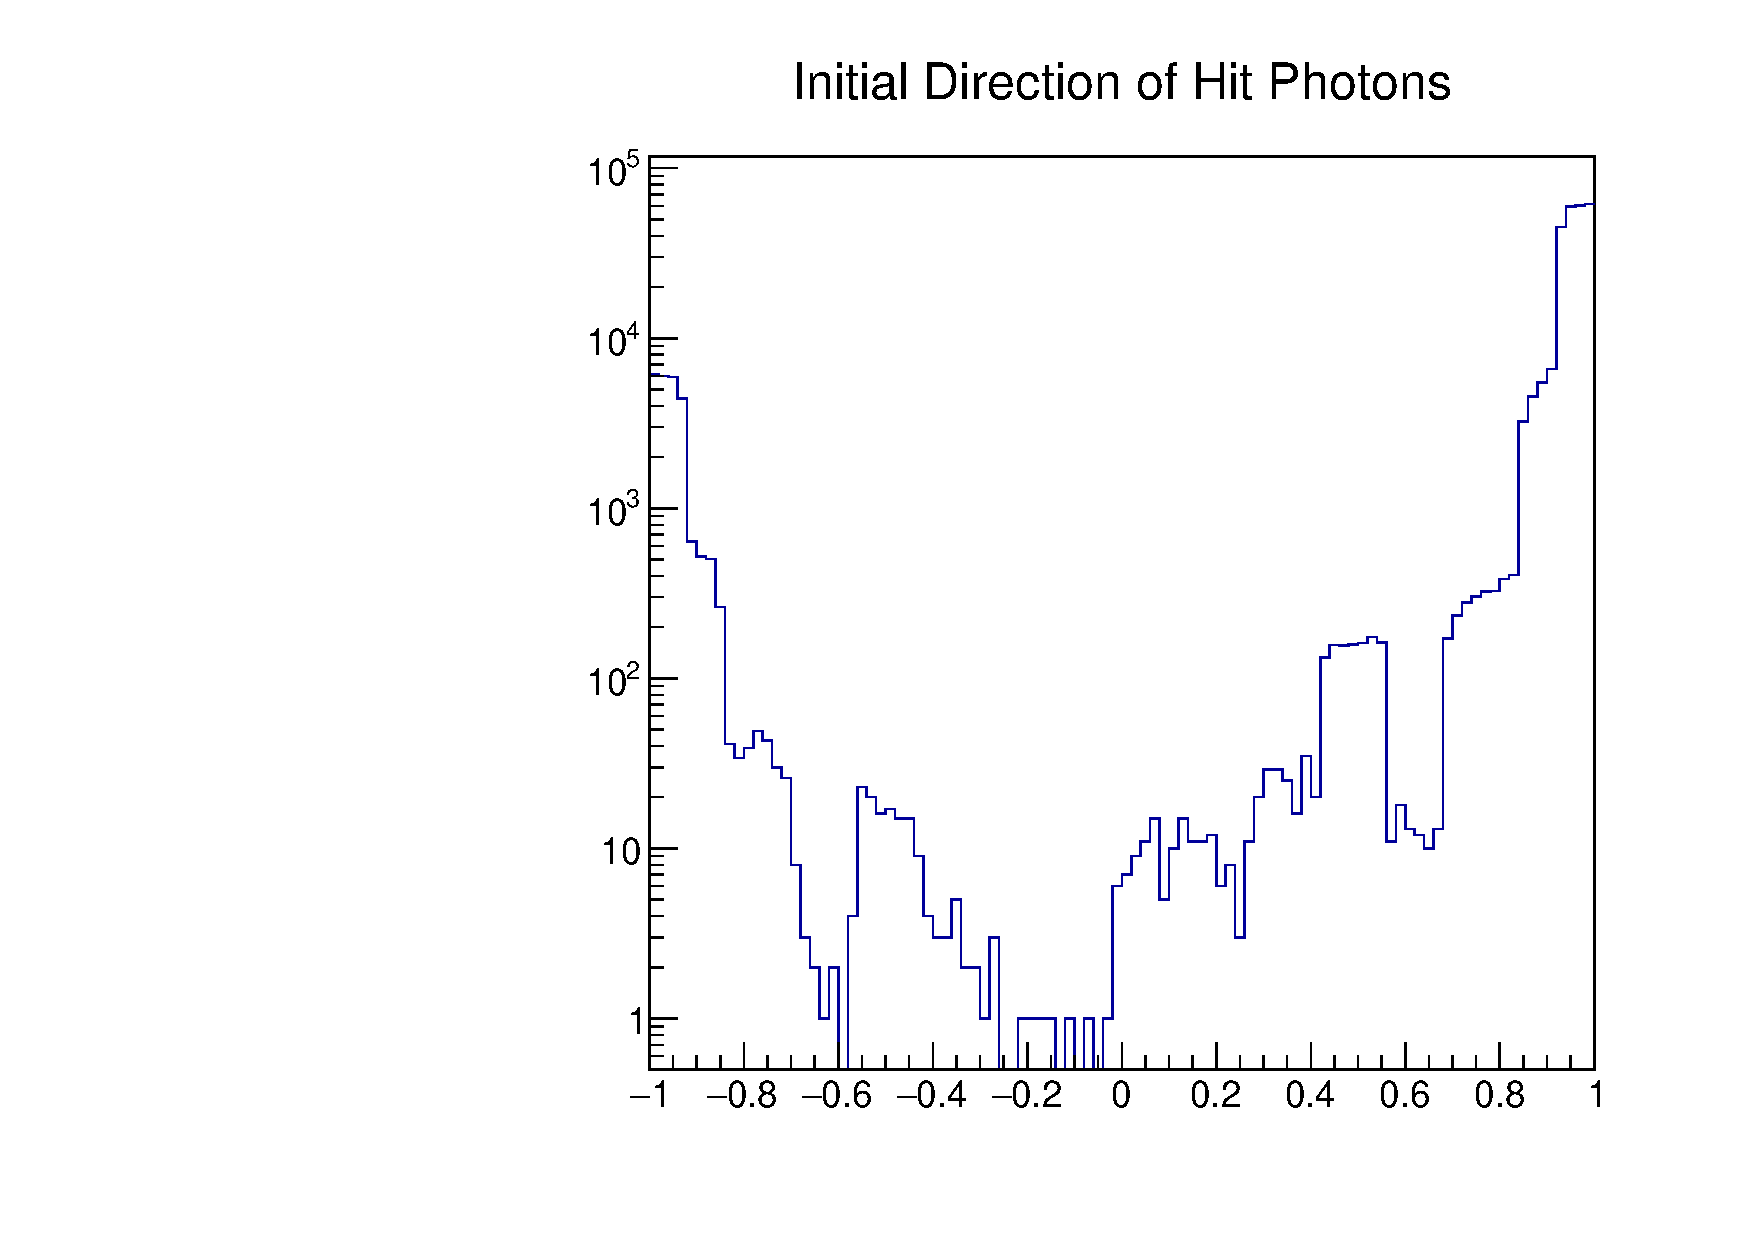
\includegraphics[width=1.0\textwidth]{figures/init_0.pdf}
		\end{minipage}
		\caption{$r=0$mm}
	\end{subfigure}
	\begin{subfigure}{0.32\textwidth}
		\begin{minipage}{1.0\textwidth}
			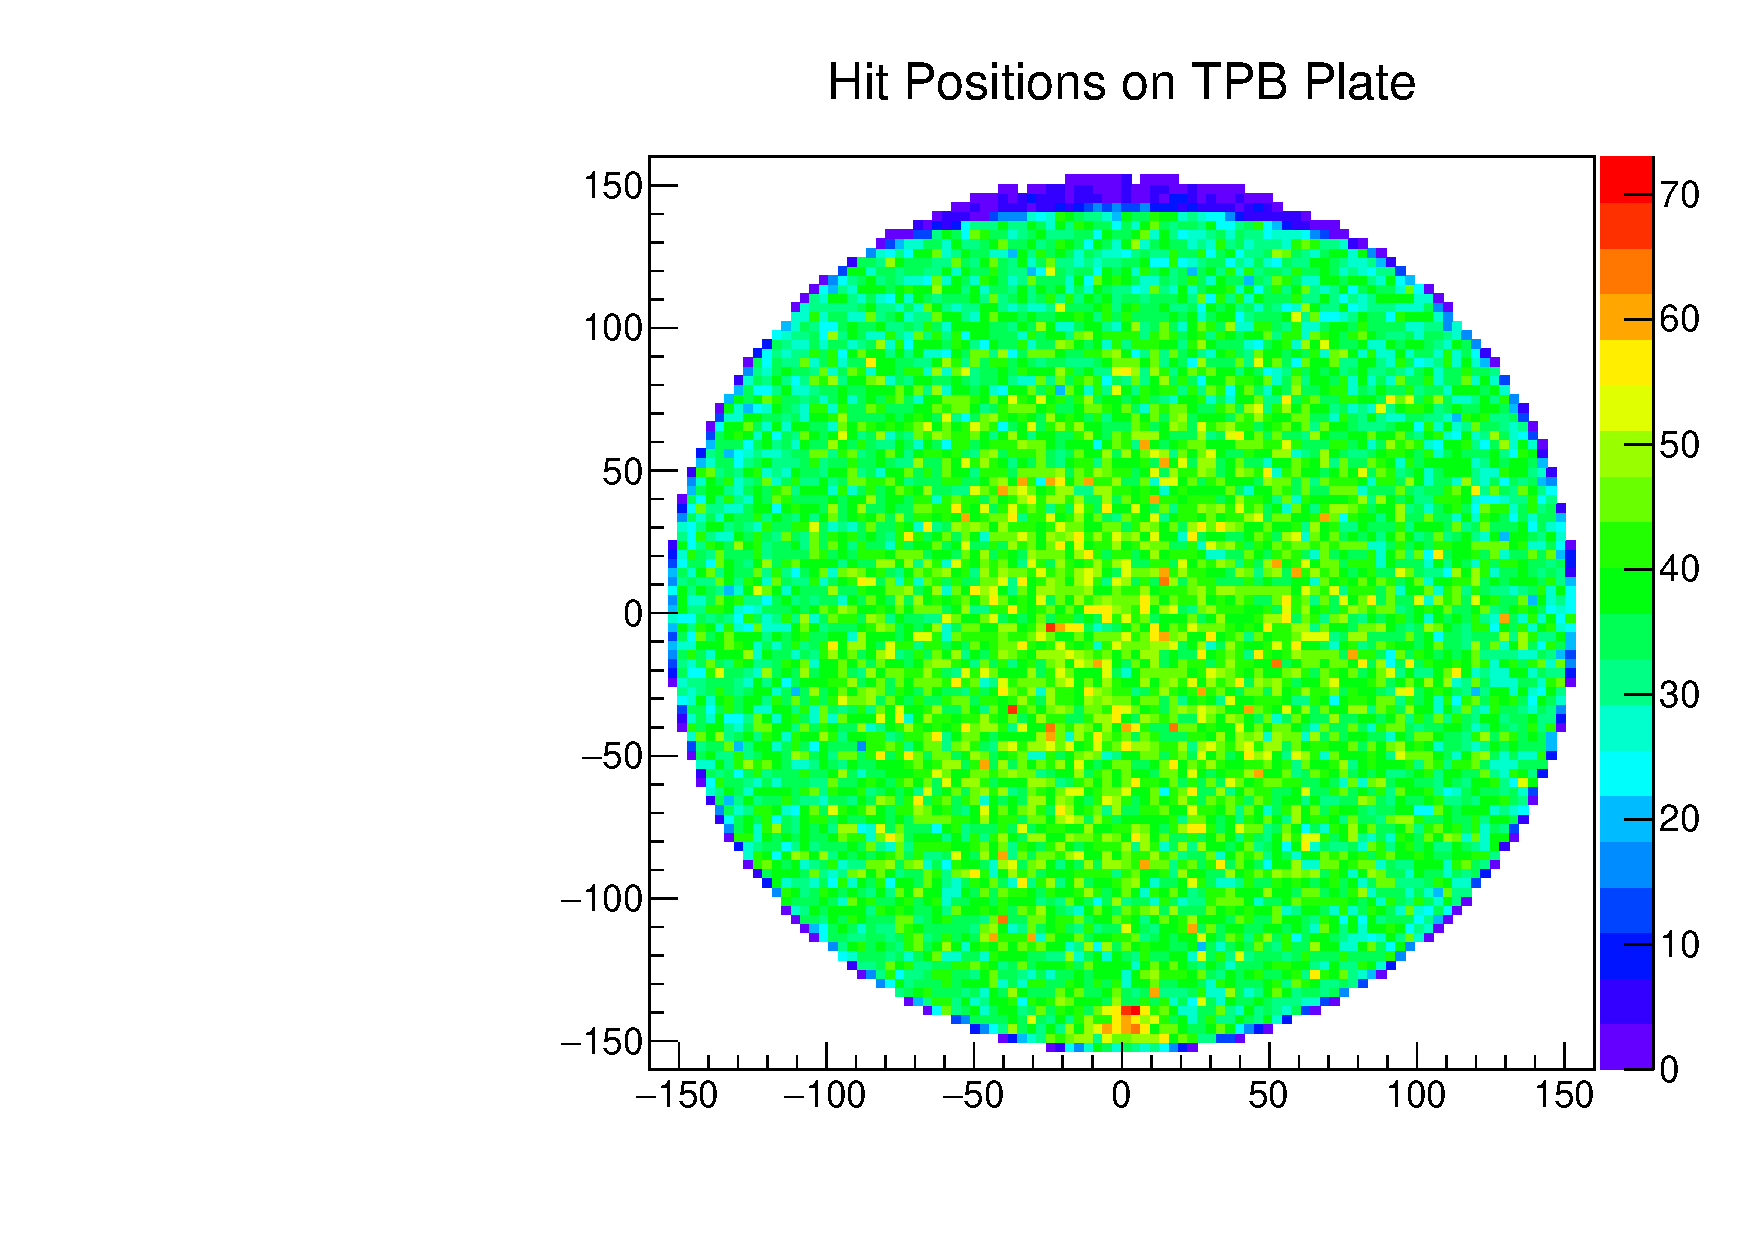
\includegraphics[width=1.0\textwidth]{figures/hit_100.pdf}
			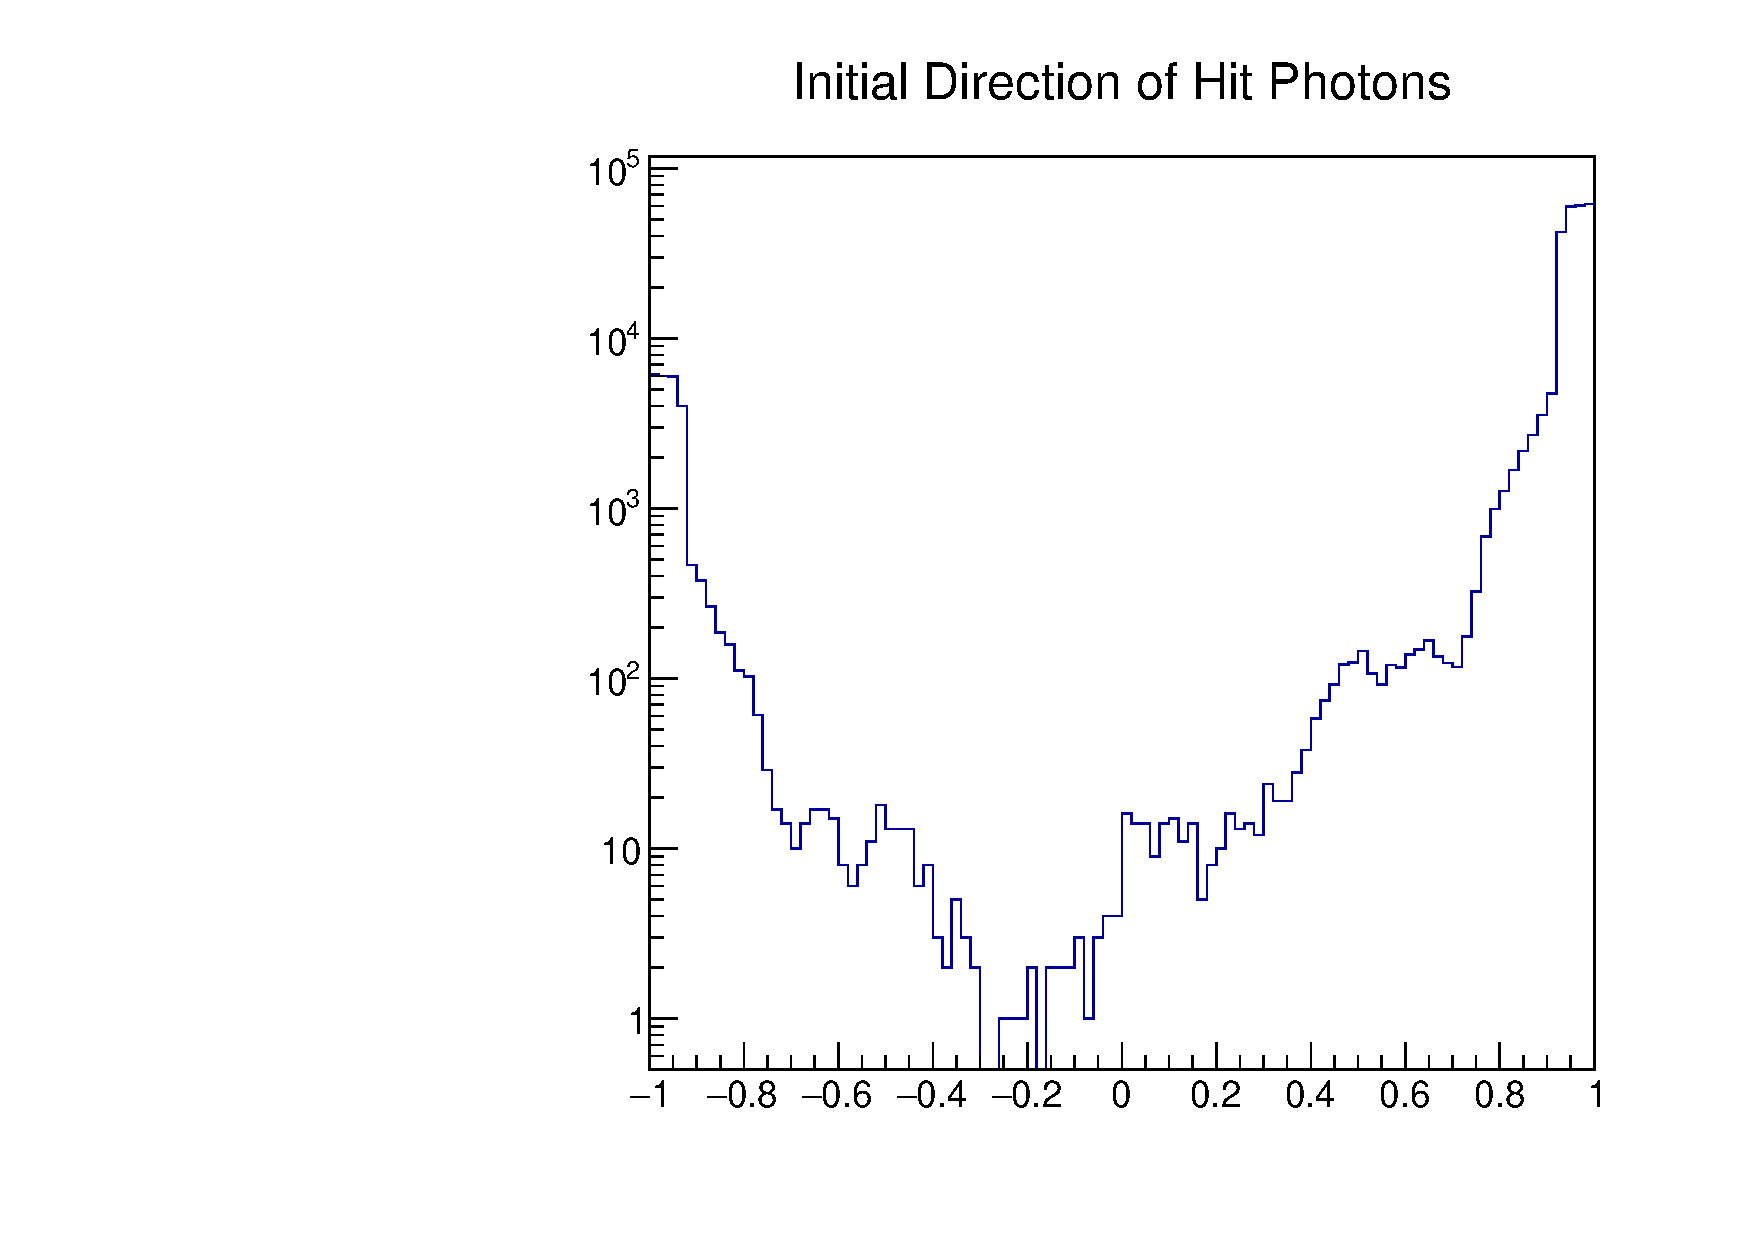
\includegraphics[width=1.0\textwidth]{figures/init_100.pdf}
		\end{minipage}
		\caption{$r=1$mm}
	\end{subfigure}
	\begin{subfigure}{0.32\textwidth}
		\begin{minipage}{1.0\textwidth}
			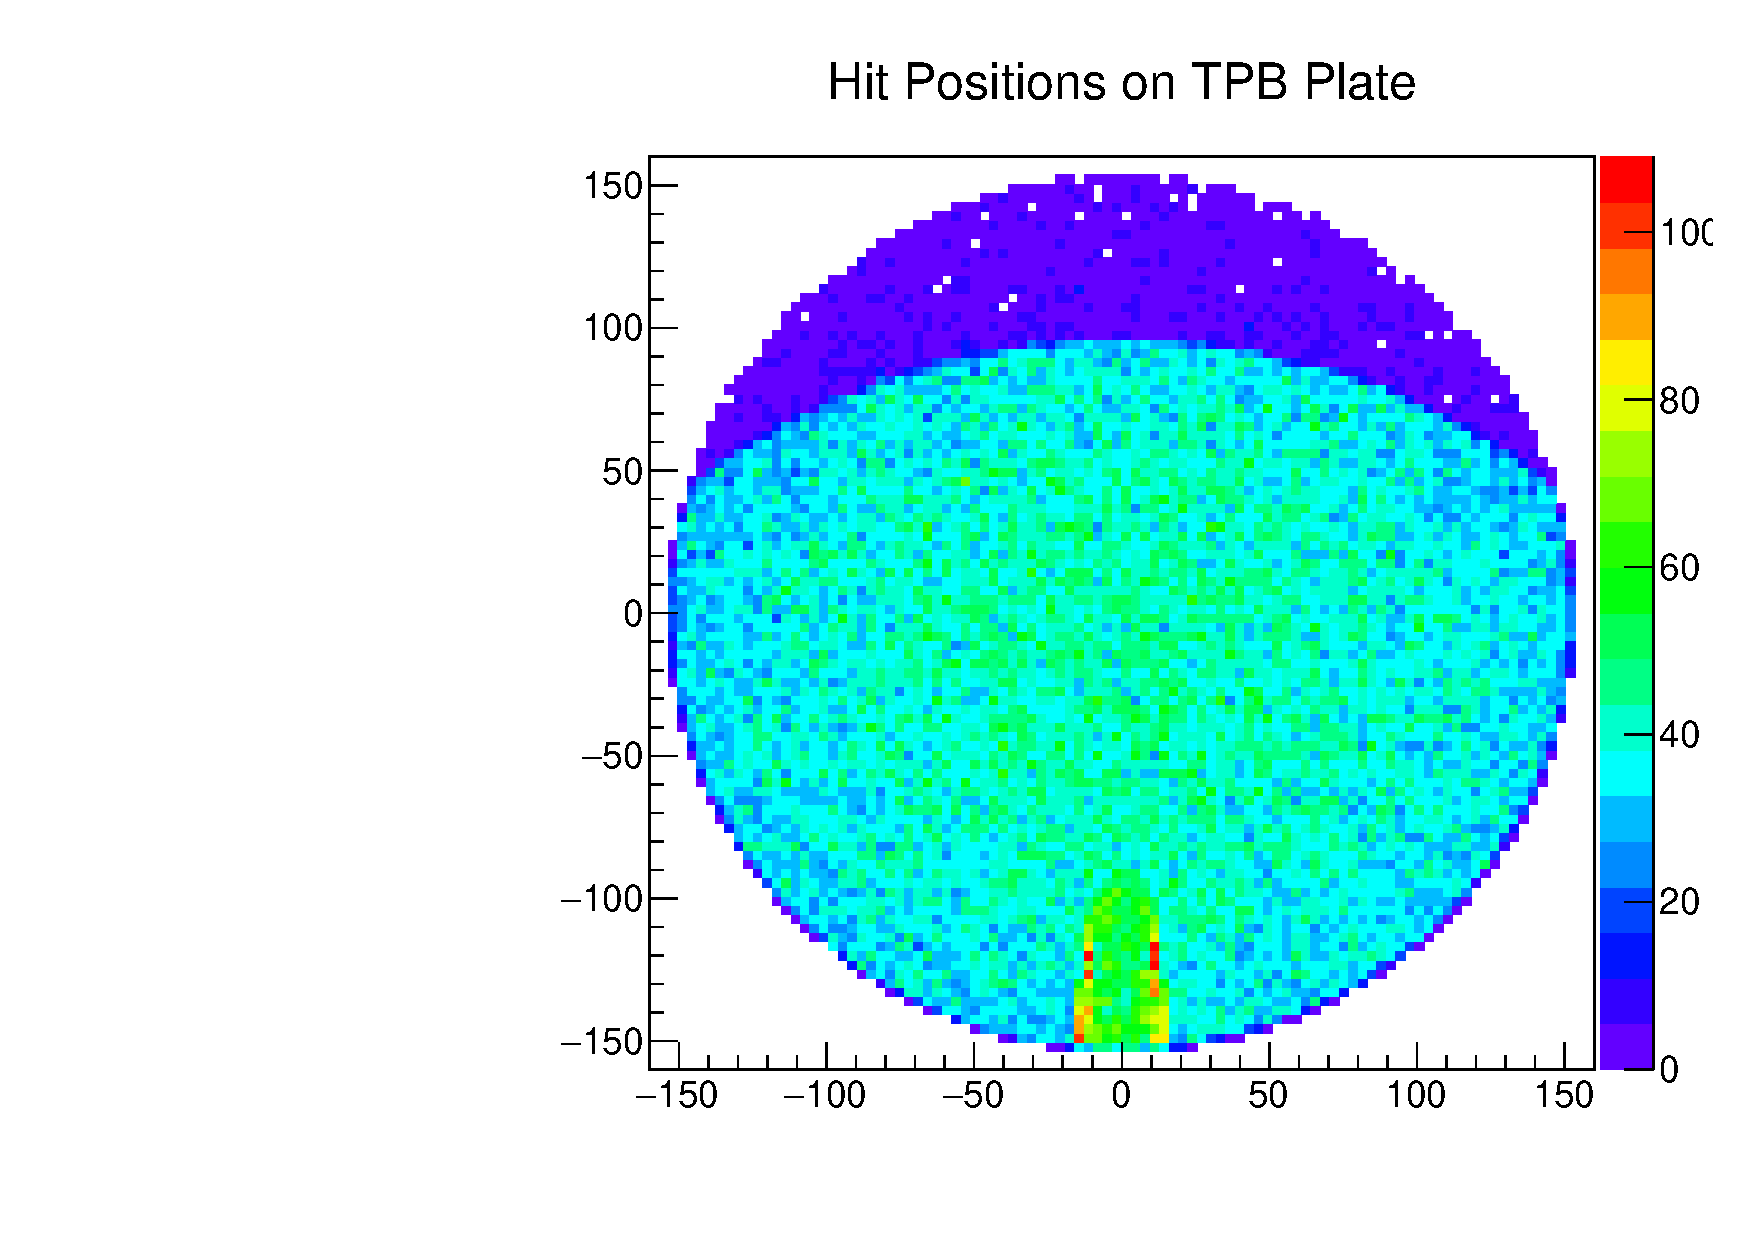
\includegraphics[width=1.0\textwidth]{figures/hit_150.pdf}
			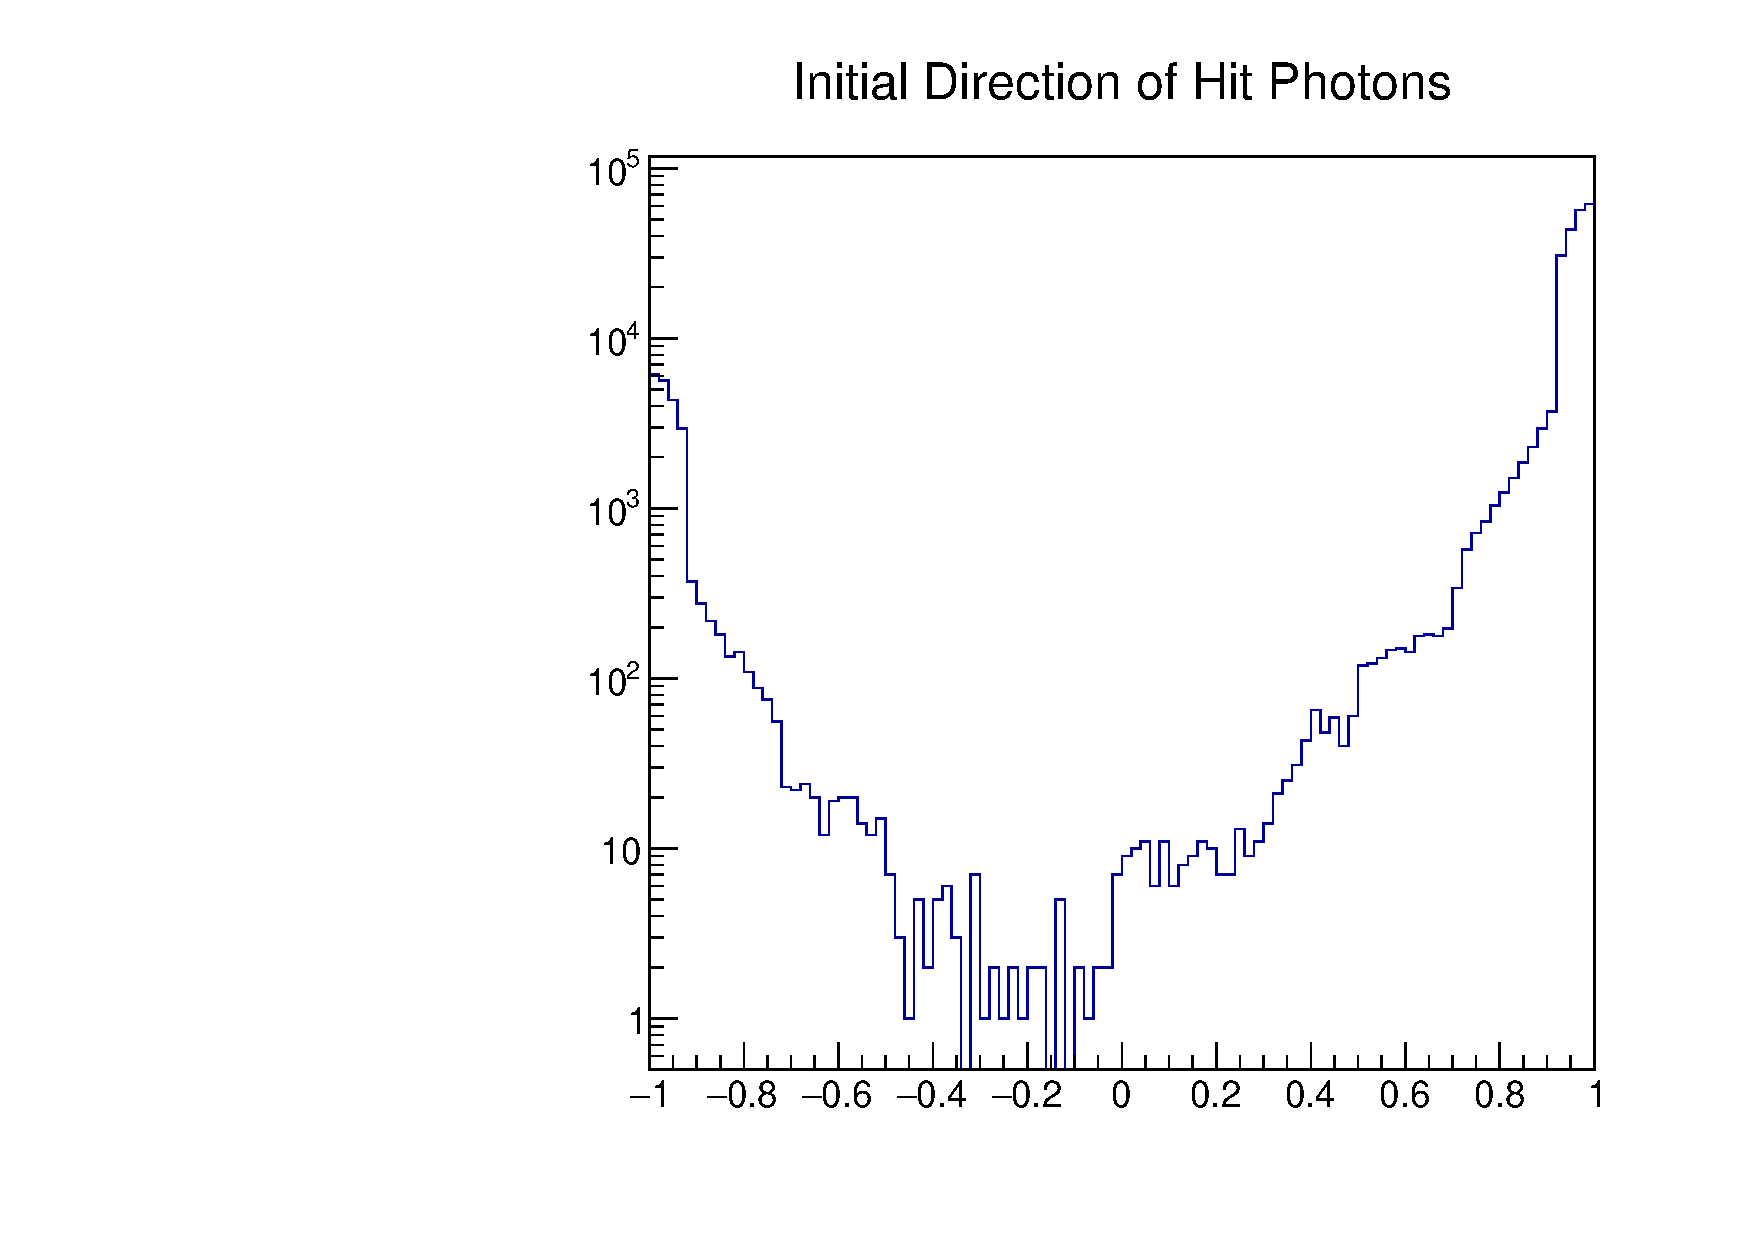
\includegraphics[width=1.0\textwidth]{figures/init_150.pdf}
		\end{minipage}
		\caption{$r=1.5$mm}
	\end{subfigure}
	\end{center}
	\caption{Plots associated with $d=36.8$cm. Top row: Hit positions on the TPB plate (units mm) as a function of the source position in the source holder, $r$, showing eclipsing as the source is moved behind the outer collimator cylinder. Bottom row: Initial directions ($\cos \theta_0$) of hitting photons. \label{fig:hitpos}} 
\end{figure}

The full simulation involves the combination of weighting several steps.

\begin{enumerate}
	\item The probability of a 420 nm photon created in the TPB plate registering as a hit on the PMT is found as a function of hit position on the plate. In RAT, a point source is placed at a fixed depth in the TPB plate, and moved along the radius of the TPB plate in steps. At each step, a number of photons is generated and tracked through to the PMT. The number of photons that register as hits on the PMT, divided by the total number of photons generated at each radial position gives the efficiency curve shown in Figure \ref{fig:plt2pmt} (left).
	
	\item The distribution of hits on the TPB plate is found as a function of starting position in the source holder Several sample distributions are shown in Figure \ref{fig:hitpos}. In this step, 128 nm photons are created in the aluminum source holder and propagate through the liquid argon volume. The positions of photons that hit the TPB plate are saved and convolved with (1). The convolution is done by calculating the distance from each hit position to the center of the TPB plate, and linearly interpolating along the curve shown in Figure \ref{fig:plt2pmt} (left) to compute a ``weighted hit''. The weighted hits are summed to give the mean number of photons registered on the PMT at each source position. This is shown in Figure \ref{fig:plt2pmt} (right), in units of photoelectrons. The multiplicative factors used to convert weighted hits into PE are:
	
	\begin{itemize}
		\item $1.18 \pm 0.1$ efficiency of 128 nm light re-emitting 420 nm light in the TPB plate, coated via evaporation.
		\item $0.64$ relative efficiency of the plate to our own plate, which is dipped in TPB instead of coated via evaporation.
		\item $0.199$ quantum efficiency of the MicroBooNE PMTs
	\end{itemize}
	
	Finally, we expect $134000 \pm 6000$ photons per alpha decay. We scale the final number of PEs by the ratio of this number to the number of simulated photons.
	
	\item To generate an expected photoelectron spectrum, we convolve the curves shown in Figure \ref{fig:plt2pmt} (right) with a simple Monte Carlo. Points are randomly selected within the area of the source disk following a bivariate normal distribution with $x$ and $y$ positions independent, and $\sigma=$. The distance from each point to the source disk origin is calculated, and the corresponding photoelectrons at that distance are computed by linearly interpolating along the curves from Figure \ref{fig:plt2pmt} (right).  The last step is to simulate a Poisson process governing the PE distributions. The results of this step are shown in Figure \ref{fig:pedist}.
\end{enumerate}

\begin{figure}
	\begin{minipage}{0.49\textwidth}
		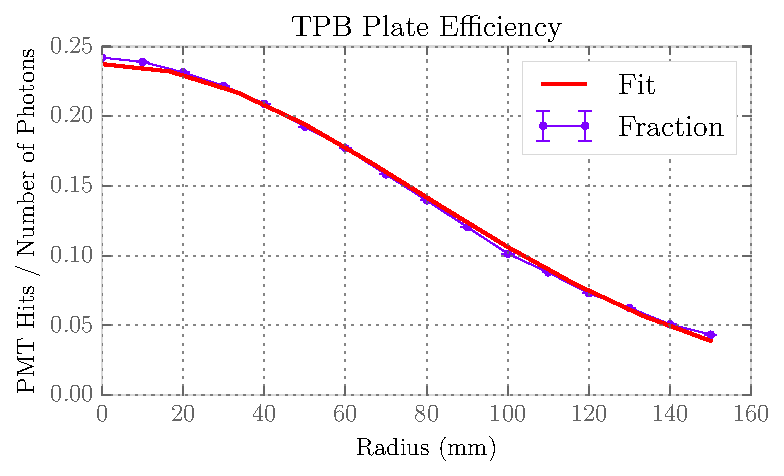
\includegraphics[width=1.0\textwidth]{figures/plt2pmt}
	\end{minipage}
	\begin{minipage}{0.49\textwidth}
		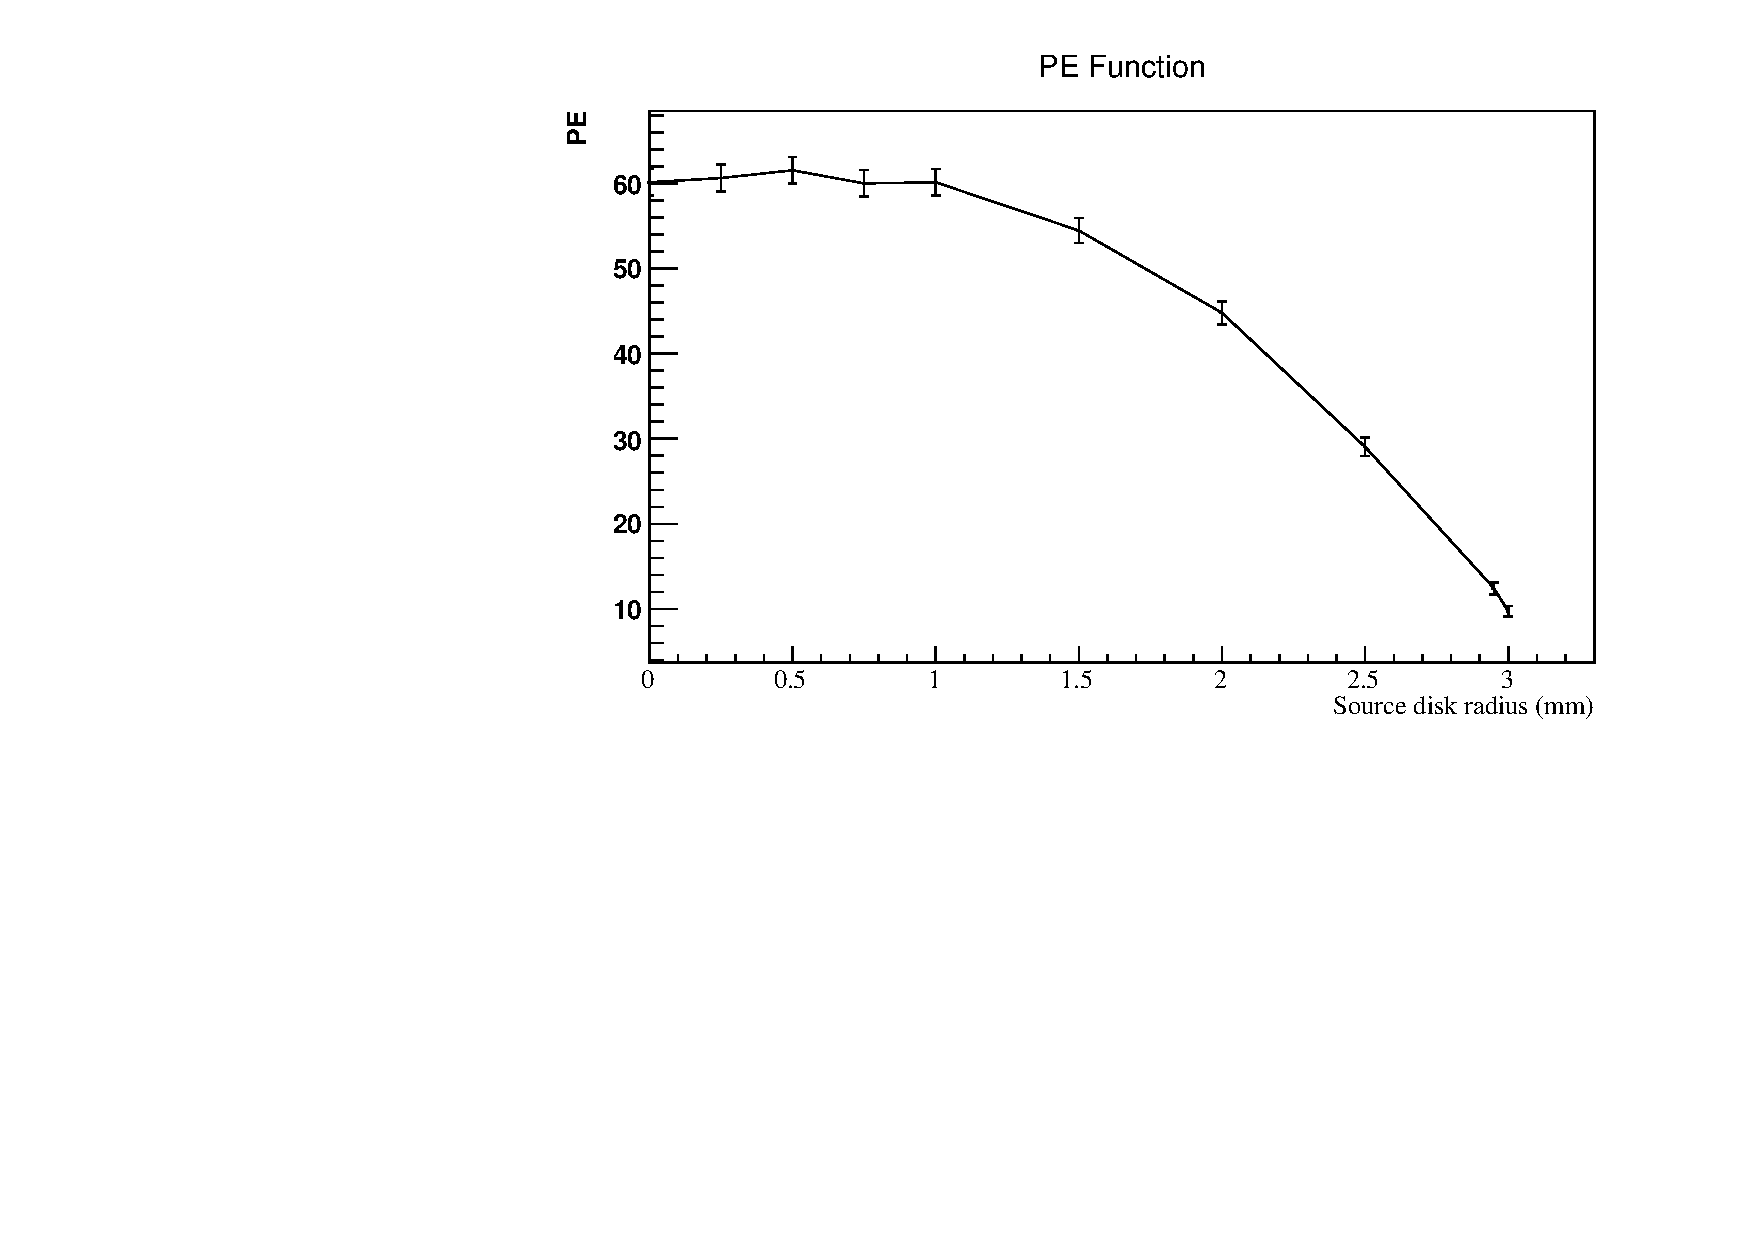
\includegraphics[width=1.0\textwidth]{figures/pefunct}
	\end{minipage}
	\caption{Left: Percentage of 420 nm photons produced in the TPB plate which reach the PMT. The red curve is a Gaussian fit, with $\sigma = 80$. Right: photoelectrons as a function of source position in the source holder, for both $d=20.3$ and $d=36.8$.\label{fig:plt2pmt}}
\end{figure}

\begin{figure}
	\begin{minipage}{0.49\textwidth}
		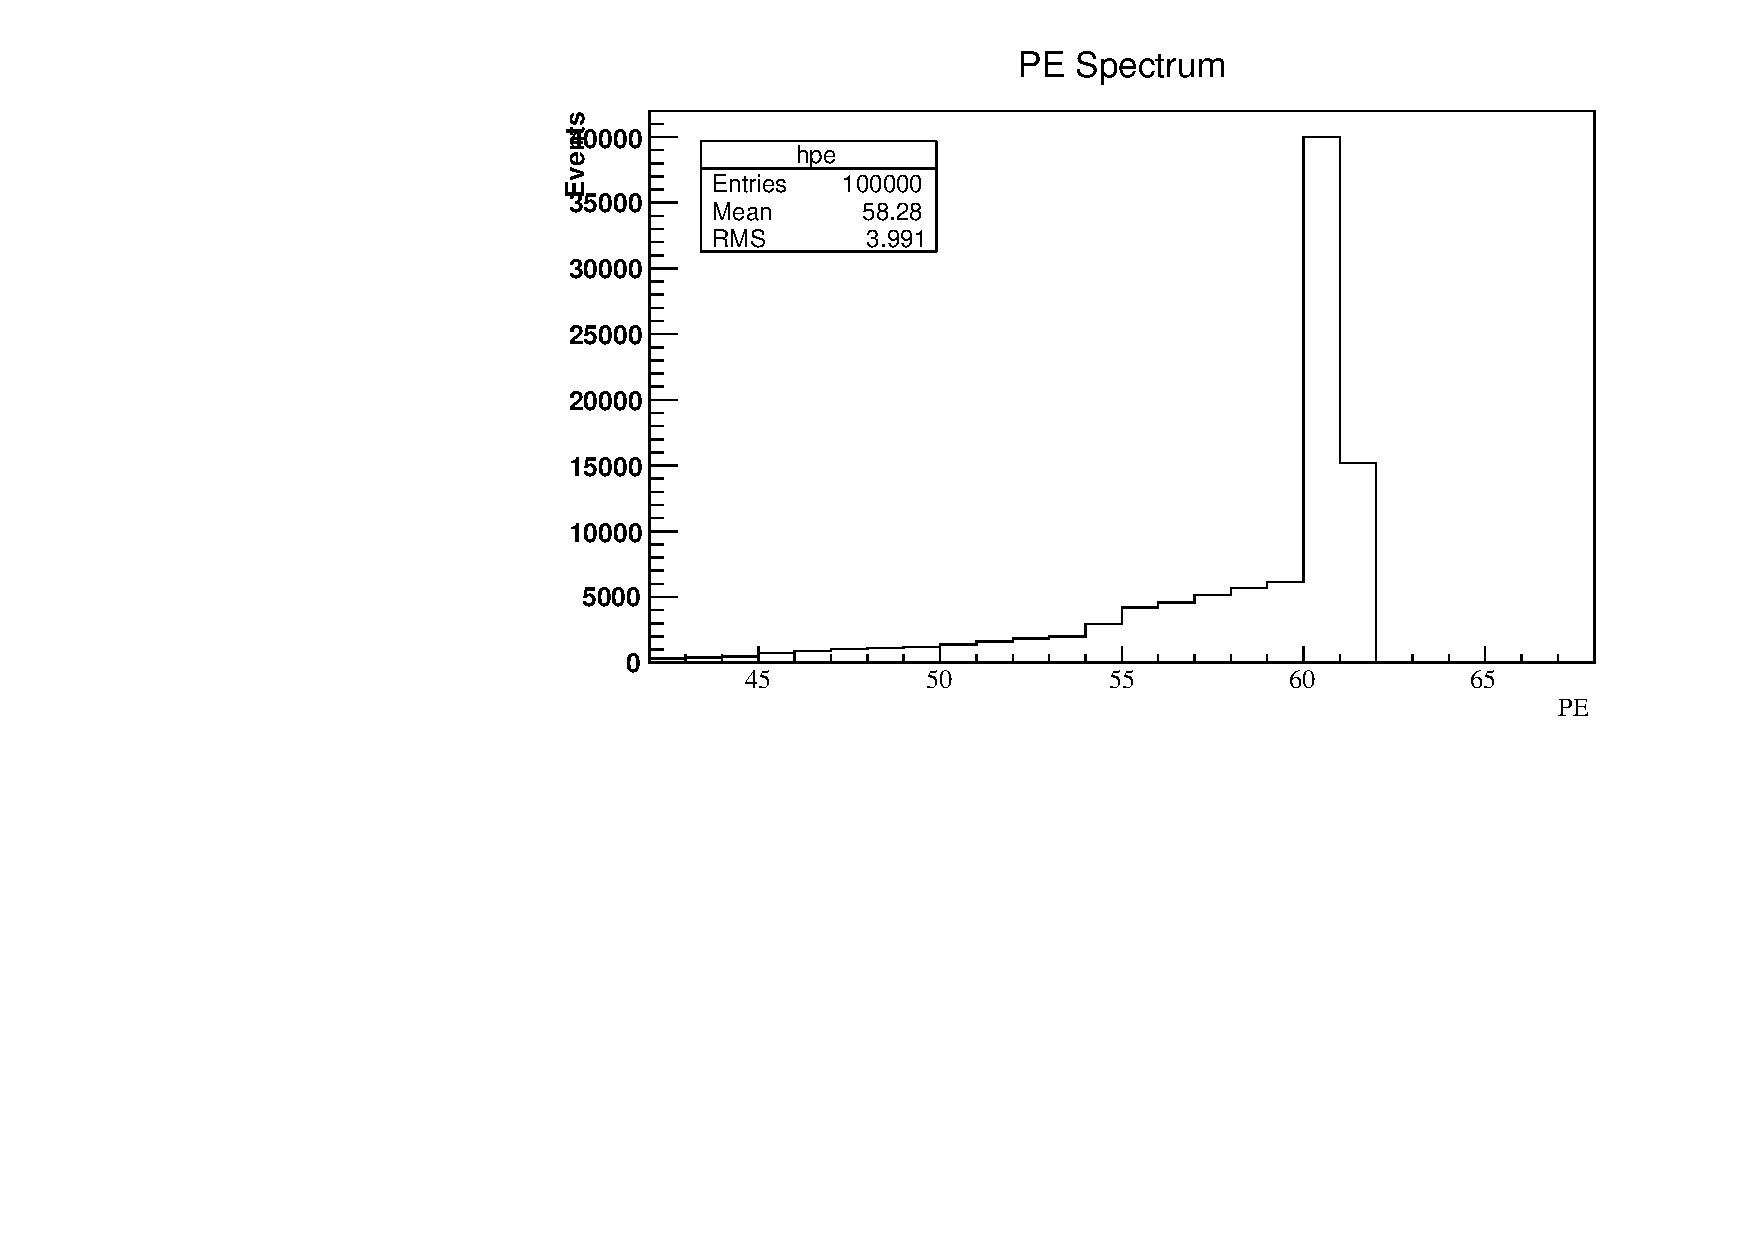
\includegraphics[width=1.0\textwidth]{figures/rawpe}
	\end{minipage}
	\begin{minipage}{0.49\textwidth}
		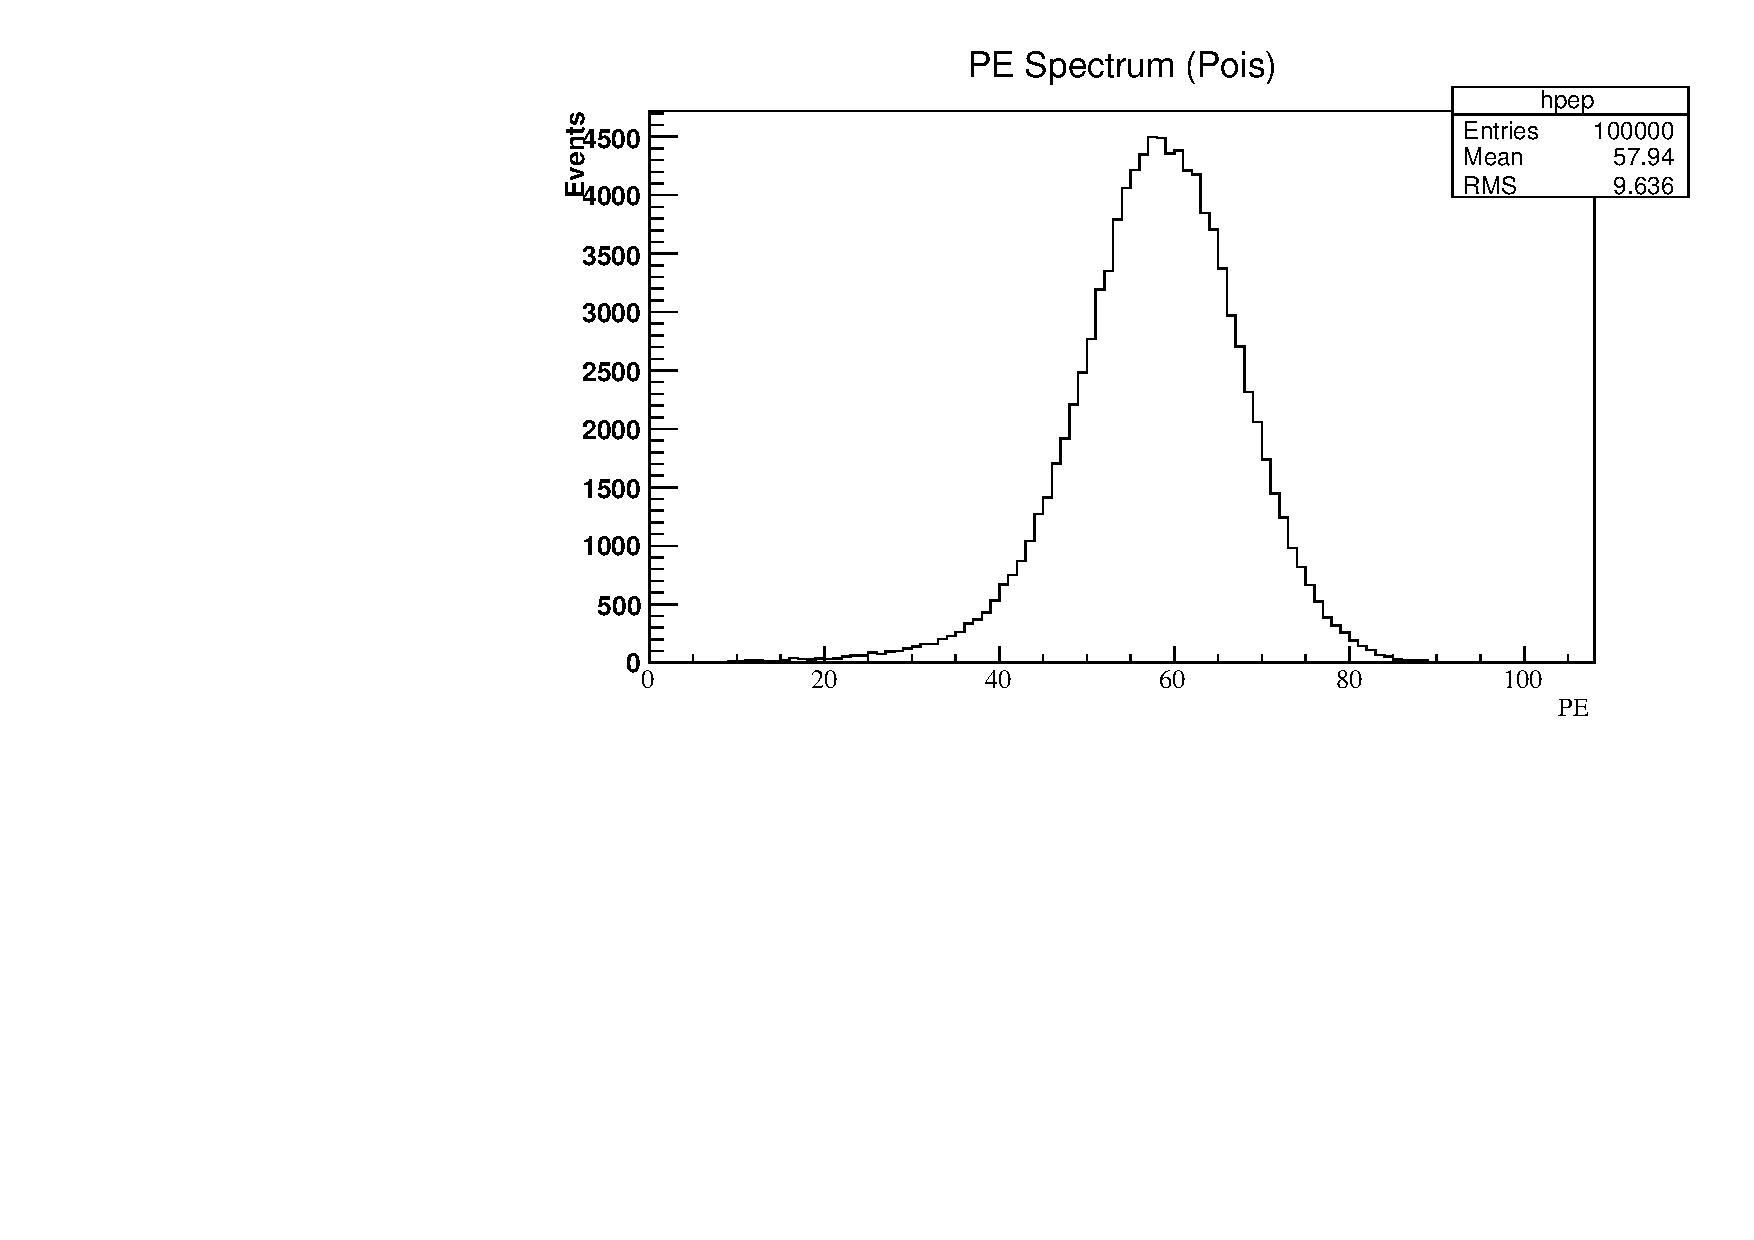
\includegraphics[width=1.0\textwidth]{figures/poispe}
	\end{minipage}
	\caption{Left: Distribution of PE from source emission Monte Carlo. Left: Poisson-smeared distribution, showing the observed PE peak.\label{fig:pedist}}
\end{figure}

%\begin{figure}
%	\begin{center}
%		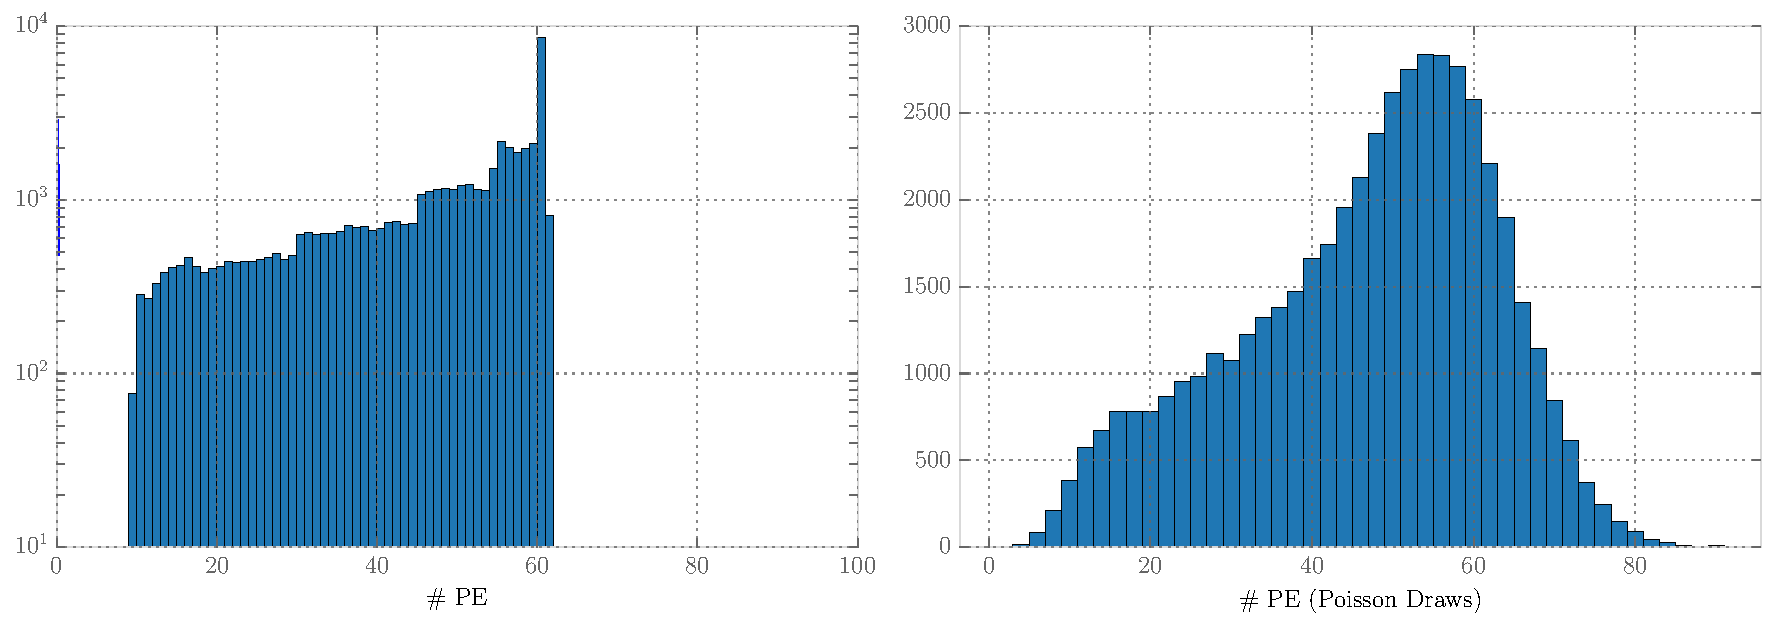
\includegraphics[width=1.0\textwidth]{figures/pedist}
%	\end{center}
%	\caption{Left: Distribution of PE from source emission Monte Carlo. Left: Poisson-smeared distribution, showing the observed PE peak.\label{fig:pedist}}
%\end{figure}

The final PE spectrum from (1)-(2)-(3) above can be fitted to obtain the expected number of observed PE for a given distance. The results of running the full simulation, and fitting the final PE spectrum, using the nominal simulation parameters are presented in Table \ref{tab:nomvals}. The final list of all parameter nominal values and uncertainties is outlined in Table \ref{tab:system}. 

\begin{table}
	\begin{center}
		\begin{tabular}{| c | c | c | c |}
			\hline
			$d$	(cm) &	PE	&	Plate Hits	&	$\langle Q \rangle$ \\
			\hline
			20.3	&	166.6	&	&	\\
			36.8	&	58.8	&	& \\
			\hline
		\end{tabular}
	\end{center}
	\caption{Summary of simulation results, using the nominal values summarized in \ref{tab:system}. Note that the number of plate hits is scaled based on the simulation size, so that PE and plate hits can be compared to experimental values. $\langle Q \rangle$ is the ratio, via Equation \ref{eq:gqe}. \label{tab:nomvals}}
\end{table}

\subsection{Systematic Errors}\label{ssec:system}

The RAT simulation is sensitive to some parameters and insensitive to others. Following the analysis steps outlined previously, the full RAT simulation is run several times, varying each parameter by its estimated $1$-$\sigma$ value. The change in the number of PE due to changing each parameter by its $1$-$\sigma$ value is summarized in Table \ref{tab:system}. Note that absolute values are taken, and that these tests were done by testing the upper limits only.

\begin{table}
	\begin{center}
		\begin{tabular}{| c | c | c | c | c | c |}
			\hline
			\textbf{Parameter} & \textbf{Value} & \textbf{1-$\sigma$} & \textbf{PE, $d=20.3$} & \textbf{PE, $d=36.8$} & \textbf{\% Change}\\
			\hline
			Source Distribution Width	&	0.08mm	&	$\pm 0.07$mm	&	155.3	&		&	6.8\\
			Source Height in Holder	&	0.01cm	&	$\pm 0.002$cm	&	165.8	&	58.7	& 0.33	\\
			\hline
			$N_{\text{LAr}}$, 128 nm	&	1.45	&	$\pm 0.07$	&	& 61.8	& 5.1\\
			$N_{\text{LAr}}$, 420 nm	&	1.23	&	$\pm 0.002$	&	&	58.8	& 0\\
			$N_{\text{Acrylic}}$, 420 nm	&	1.49	&	$\pm 0.02$	&	153.2	&	&	8.04 \\
			$N_{\text{Glass}}$, 420 nm	&	1.46	&	$\pm 0.04$	&	& 57.8	& 1.7\\
			$R_{\text{Al}}$, 128 nm	&	0.1	&	+0.2	&	234.1	&	& \color{red}{41} \\
			$R_{\text{Al}}$, Type	&	Specular	&	Diffuse	&	&	59.3	& 0.85\\
			$R_{\text{Stainless}}$, 128 nm	&	0.35	&		&	&	& \\
			$R_{\text{Stainless}}$, 420 nm	&	0.540	&	$\pm 0.005$	&	167.5	&	& 0.54\\
			$R_{\text{Stainless}}$, Type	&	Specular	&	Diffuse	&	&	59.4	& 1.02\\
			\hline
			$d$	&	20.3/36.8cm	&	4mm	&	&	& \\
			Collimator Width 1	&	2.5mm	&	$+0.07^*$	&	169.1	&	59.1	& 1.01\\
			Collimator Width 2	&	3.0mm	&	$+0.18^*$	&	-	&	-	& \\
			Collimator Height	&	0.15625in	&	$-0.025$in	&	&	& \\
			Plate to PMT Distance	&	0.125in	&	$\pm 0.03$in	&	159.7	&	& 4.1\\
			Glass Thickness	&	0.5cm	&		&	&	59.0	& 0.34\\
			\hline
			Evap. TPB Efficiency	&	1.18	&	$\pm 0.1$	&		&		&	8.5\\
			Rel. Efficiency to Evap. TPB	&	0.64	&		&		&		&	\\
			PMT Quantum Efficiency	&	0.199	&		&		&		&	\\
			$N_{\gamma}$, Alpha	&	134000	&	$\pm 6000$	&		&		&	4.4 \\
			\hline
			\hline
			\textbf{Quadrature Sum}	&	-	&	-	&	-	&	-	&	$15.9$	\\
			\textbf{Nominal Sim. Values}	&	-	&	-	&	166.6	&	58.8	&	-	\\
			\textbf{Data}	&	-	&	-	&	74.1	&	28.5	&	-	\\
			\hline
		\end{tabular}
		\caption{Summary of systematic uncertainty sources in the RAT simulation, as they relate to the nominal PE value. The parameters are grouped by source positioning, material parameters, geometry parameters, and multiplicative factors. PE values computed with each parameter set to the $+1$-$\sigma$ value. \hfill \\ $^*$Vary together.\label{tab:system}}
	\end{center}
\end{table}

% Create the reference section using BibTeX:
\bibliography{ref}

\end{document}
%
% ****** End of file apstemplate.tex ******
